\documentclass[pdftex,12pt,xcolor=svgnames]{beamer}

\mode<presentation>
{
  \usetheme{boxes}
  \usecolortheme[named=MidnightBlue]{structure}
  %\setbeamercolor{normal text}{bg=NavajoWhite!20}
  \usefonttheme{serif}
  \setbeamertemplate{navigation symbols}{}
  % Show frame number and author name in footline
  \setbeamertemplate{footline}[frame number]
  \addtobeamertemplate{footline}{\quad\textcolor{gray}{James Robert Lloyd}}{}
  % Set frame titles in small capitals
  \setbeamerfont{frametitle}{shape=\scshape,family=\rmfamily}
  \setbeamercolor{frametitle}{bg=gray!60!white,fg=black}
  % Alerted text: blue (uncomment second line if theme sets alerted text to bold)
  \setbeamercolor{alerted text}{fg=blue}
  %\setbeamerfont*{alerted text}{}
  \setbeamertemplate{bibliography item}[text] %{\hbox{\donotcoloroutermaths$\blacktriangleright$}}
  \setbeamertemplate{bibliography entry title}{}
  \setbeamertemplate{bibliography entry author}{}
  \setbeamertemplate{bibliography entry note}{}
  \setbeamertemplate{bibliography entry location}{}

}
\usepackage[english]{babel}
\usepackage[latin1]{inputenc}
\usepackage{times}
\usepackage[T1]{fontenc}
\usepackage{hyperref}
\usepackage{multimedia}
\usepackage{eepic}
\usepackage{graphicx}
%\usepackage[nohug]{latexinclude/diagrams}
\usepackage{tikz}
\usetikzlibrary{calc}

%% \newcommand{\footlineextra}[1]{
%%     \begin{tikzpicture}[remember picture,overlay]
%%         \node[yshift=1.5ex,anchor=south east] at (current page.south east)
%% {#1};
%%     \end{tikzpicture}
%% }

\newcommand{\footlineextra}[1]{
    \begin{tikzpicture}[remember picture,overlay]
        \node[xshift=-5ex,yshift=-0.5ex,anchor=south east] at (current page.south east)
             {\mbox{\tiny \textcolor{MidnightBlue}{#1}}};
    \end{tikzpicture}
}

\def\sectionframe#1{
  {
    \setbeamertemplate{footline}{\empty}
    \begin{frame}{}
      \begin{center}
        \huge\sc #1
      \end{center}
    \end{frame}
  }
}


\usepackage{etex}

\usepackage{tabularx}
\usepackage{include/picins}
\usepackage{include/preamble}
\usepackage{xcolor}
\usepackage{tikz}

\usetikzlibrary{shapes.geometric,arrows,chains,matrix,positioning,scopes,calc}

%%%%%%%%%%%%%%%%%%%%%%%%%%%%%%%%%%%%%%%%%%%
%
% Some look and feel definitions
%
%%%%%%%%%%%%%%%%%%%%%%%%%%%%%%%%%%%%%%%%%%%

\setlength{\columnsep}{0.03\textwidth}
\setlength{\columnseprule}{0.0018\textwidth}
\setlength{\parindent}{0.0cm}
  
\tikzstyle{mybox} = [draw=white, rectangle]
\tikzset{hide on/.code={\only<#1>{\color{white}}}}

\definecolor{camlightblue}{rgb}{0.601 , 0.8, 1}
\definecolor{camdarkblue}{rgb}{0, 0.203, 0.402}
\definecolor{camred}{rgb}{1, 0.203, 0}
\definecolor{camyellow}{rgb}{1, 0.8, 0}
\definecolor{lightblue}{rgb}{0, 0, 0.80}
\definecolor{white}{rgb}{1, 1, 1}
\definecolor{whiteblue}{rgb}{0.80, 0.80, 1}

\newcolumntype{x}[1]{>{\centering\arraybackslash\hspace{0pt}}m{#1}}
\newcommand{\tabbox}[1]{#1}

\hypersetup{colorlinks=true,citecolor=blue}

%%%%%%%%%%%%%%%%%%%%%%%%%%%%%%%%%%%%%%%%%%%
%
% The talk
%
%%%%%%%%%%%%%%%%%%%%%%%%%%%%%%%%%%%%%%%%%%%

\title{How to build an automatic statistician}

\author{
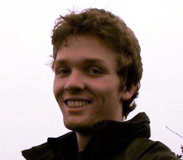
\includegraphics[height=0.2\textwidth]{figures/JamesLloyd4}
\qquad
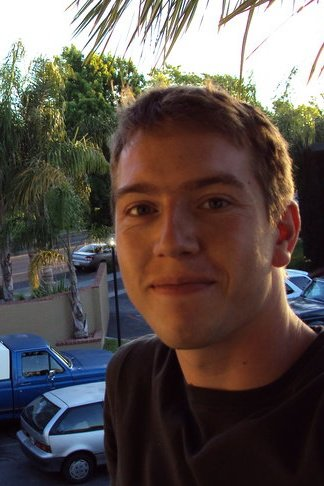
\includegraphics[height=0.2\textwidth, trim=20mm 25mm 0mm 25mm, clip]{figures/david2}
\qquad
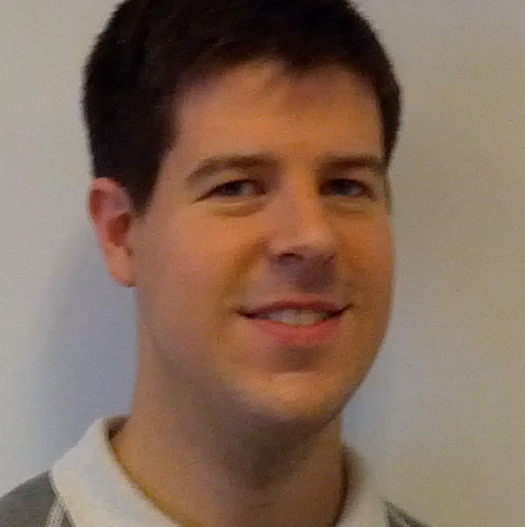
\includegraphics[height=0.2\textwidth]{figures/roger-photo}
\\
James Robert Lloyd\textsuperscript{1}, David Duvenaud\textsuperscript{1}, Roger Grosse\textsuperscript{2},\\
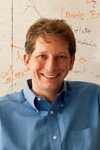
\includegraphics[height=0.2\textwidth, trim=0mm 7mm 0mm 0mm, clip]{figures/josh2}
\qquad
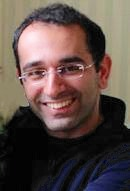
\includegraphics[height=0.2\textwidth]{figures/zg2}\\
Joshua Tenenbaum\textsuperscript{2}, Zoubin Ghahramani\textsuperscript{1}
}

\institute{
1: Department of Engineering, University of Cambridge, UK\\2: Massachusetts Institute of Technology, USA
}

\begin{document}

\frame[plain] {
\titlepage
}

\begin{frame}{There is a growing need for data analysis}
  \begin{itemize}
    \item We live in an era of abundant data
    \vspace{\baselineskip}
    \item The McKinsey Global Institute claim
    \begin{itemize}
      \item \emph{``The United States alone faces a shortage of 140,000 to 190,000 people with analytical expertise and 1.5 million managers and analysts with the skills to understand and make decisions based on the analysis of big data.''}
    \end{itemize}
    \vspace{\baselineskip}
    \item Diverse fields increasingly relying on expert statisticians, machine learning researchers and data scientists \eg
    \begin{itemize}
       \item Computational sciences (\eg biology, astronomy, \ldots)
       \item Online advertising
       \item Quantitative finance
       \item \ldots
     \end{itemize}
  \end{itemize}
\end{frame}

\begin{frame}{What would an automatic statistician do?}
    % Define block styles
  \tikzstyle{block} = [rectangle, draw, fill=blue!20, 
                       text width=4.4em, text centered, rounded corners, minimum height=3em]
  \tikzstyle{line} = [draw, -latex']
  \tikzstyle{cloud} = [draw, ellipse,fill=red!20,minimum height=2em]
    
  \begin{tikzpicture}[node distance = 2.3cm]
    \footnotesize
    % Place nodes
    \node [cloud] (data) {Data};
    \node [block, right of=data] (search) {Search};
    \node [cloud, above of=search] (language) {Language of models};
    \node [block, below of=search] (eval) {Evaluation};
    \node [cloud, right of=search] (model) {Model};
    \node [block, right of=model] (pred) {Prediction};
    \node [block, above of=pred] (trans) {Description};
    \node [block, below of=pred] (checking) {Checking};
    \node [cloud, right of=pred] (report) {Report};
    % Draw edges
    \path [line] (data) -- (search);
    \path [line] (language) -- (search);
    \path [line] (search) -- (model);
    \path [line] (search) -- (model);
    \path [line] (model.north east) -- (trans.south west);
    \path [line] (model.east) -- (pred.west);
    \path [line] (model.south east) -- (checking.north west);
    \path [line] (trans.south east) -- (report.north west);
    \path [line] (pred.east) -- (report.west);
    \path [line] (checking.north east) -- (report.south west);
    \draw[->,] (search.south east) .. controls (3.45,-1.15) .. (eval.north east);
    \draw[->,] (eval.north west) .. controls (1.15,-1.15) .. (search.south west);
  \end{tikzpicture}
\end{frame}

%\begin{frame}{Goals of the automatic statistician project}
%  \begin{itemize}
%    \item Provide a set of tools for understanding data that require minimal expert input
%    \vspace{\baselineskip}
%    \item Uncover challenging research problems in \eg
%    \begin{itemize}
%      \item Automated inference
%      \item Model construction and comparison
%      \item Data visualisation and interpretation
%    \end{itemize}
%    \vspace{\baselineskip}
%    \item Advance the field of machine learning in general
%    \vspace{\baselineskip}
%  \end{itemize}
%\end{frame}

%\begin{frame}{Ingredients of an automatic statistician}
%  \begin{center}
%    \scalebox{0.5}{  % Define block styles
  \tikzstyle{block} = [rectangle, draw, fill=blue!20, 
                       text width=4.4em, text centered, rounded corners, minimum height=3em]
  \tikzstyle{line} = [draw, -latex']
  \tikzstyle{cloud} = [draw, ellipse,fill=red!20,minimum height=2em]
    
  \begin{tikzpicture}[node distance = 2.3cm]
    \footnotesize
    % Place nodes
    \node [cloud] (data) {Data};
    \node [block, right of=data] (search) {Search};
    \node [cloud, above of=search] (language) {Language of models};
    \node [block, below of=search] (eval) {Evaluation};
    \node [cloud, right of=search] (model) {Model};
    \node [block, right of=model] (pred) {Prediction};
    \node [block, above of=pred] (trans) {Description};
    \node [block, below of=pred] (checking) {Checking};
    \node [cloud, right of=pred] (report) {Report};
    % Draw edges
    \path [line] (data) -- (search);
    \path [line] (language) -- (search);
    \path [line] (search) -- (model);
    \path [line] (search) -- (model);
    \path [line] (model.north east) -- (trans.south west);
    \path [line] (model.east) -- (pred.west);
    \path [line] (model.south east) -- (checking.north west);
    \path [line] (trans.south east) -- (report.north west);
    \path [line] (pred.east) -- (report.west);
    \path [line] (checking.north east) -- (report.south west);
    \draw[->,] (search.south east) .. controls (3.45,-1.15) .. (eval.north east);
    \draw[->,] (eval.north west) .. controls (1.15,-1.15) .. (search.south west);
  \end{tikzpicture}}
%  \end{center}
%  \begin{itemize}
%    \footnotesize
%    \item {\bf An open-ended language of models}
%    \begin{itemize}
%       \item Expressive enough to capture real-world phenomena\ldots
%       \item \ldots and the techniques used by human statisticians
%     \end{itemize}
%    %\vspace{\baselineskip}
%    \item {\bf A search procedure}
%    \begin{itemize}
%       \item To efficiently explore the language of models
%     \end{itemize}
%    %\vspace{\baselineskip}
%    \item {\bf A principled method of evaluating models}
%    \begin{itemize}
%       \item Trading off complexity and fit to data
%     \end{itemize}
%    %\vspace{\baselineskip}
%    \item {\bf A procedure to automatically explain the models}
%    \begin{itemize}
%       \item Making the assumptions of the models explicit\ldots
%       \item \ldots in a way that is intelligible to non-experts
%     \end{itemize}
%  \end{itemize}
%\end{frame}

\begin{frame}{Preview: An entirely automatic analysis}

\newcommand{\wmgd}{0.5\columnwidth}
\newcommand{\hmgd}{3.0cm}
\newcommand{\mdrd}{figures/01-airline}
\newcommand{\mbm}{\hspace{-0.3cm}}
\begin{tabular}{cc}
\mbm 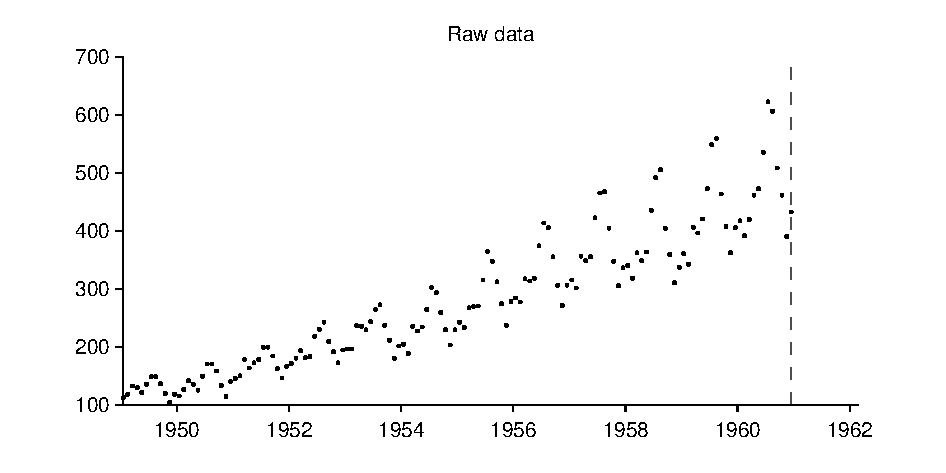
\includegraphics[width=\wmgd,height=\hmgd]{\mdrd/01-airline_raw_data} & 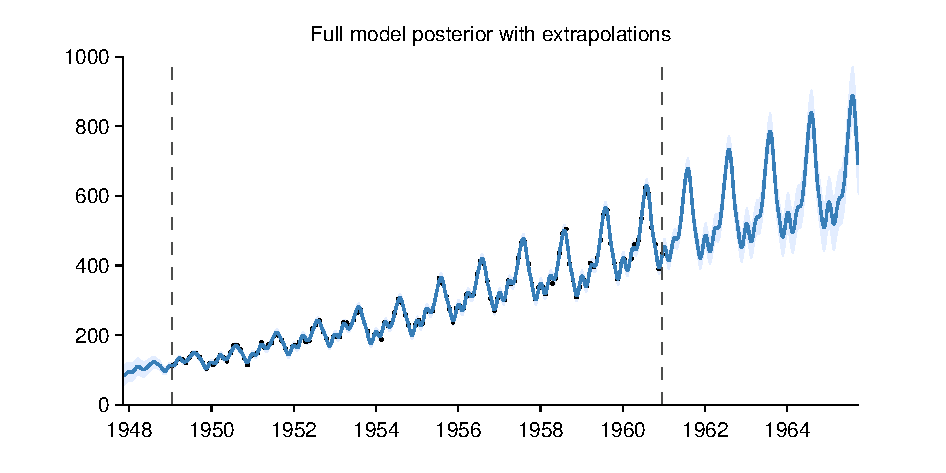
\includegraphics[width=\wmgd,height=\hmgd]{\mdrd/01-airline_all}
\end{tabular}
\vspace{0.5\baselineskip}

{\footnotesize
Four additive components have been identified in the data
\begin{itemize}

  \item A linearly increasing function. 

  \item An approximately periodic function with a period of 1.0 years and with linearly increasing amplitude. 

  \item A smooth function. 

  \item Uncorrelated noise with linearly increasing standard deviation. 

\end{itemize}
}
\end{frame}

\begin{frame}{Agenda}
  \begin{itemize}
    \item Introduction to Bayesian statistics
    \vspace{\baselineskip}
    \item Derivation of Gaussian processes via linear regression
    \vspace{\baselineskip}
    \item Description of automatic statistician
    \vspace{\baselineskip}
    \item Examples of automatically generated ouput
  \end{itemize}
\end{frame}

\begin{frame}{How to do linear regression} 
  \only<1>{
  \begin{center}
    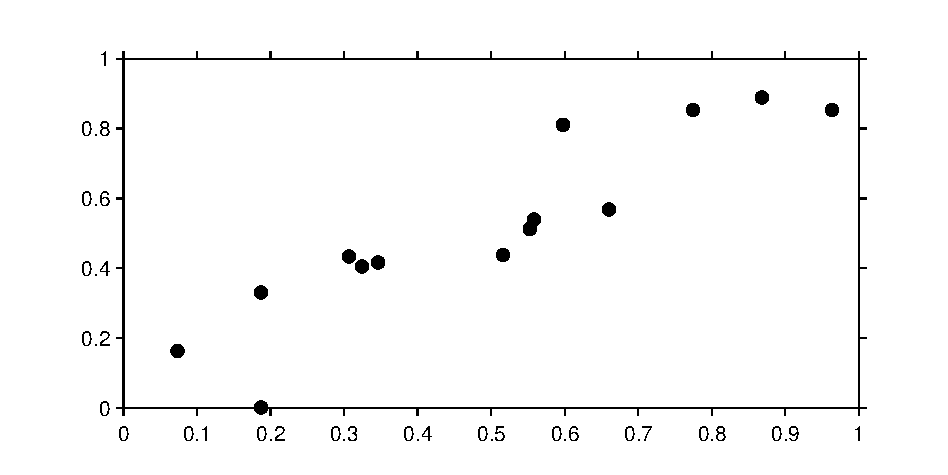
\includegraphics[width=0.8\textwidth]{figures/lin_reg/all_data}
  \end{center}
  \begin{itemize}
    \item Linear regression starts by assuming a model of the form $y_i = m x_i + \varepsilon_i$ where $x$ and $y$ are inputs and outputs respectively and $\varepsilon$ are errors or noise
  \end{itemize}
  }
  \only<2>{
  \begin{center}
    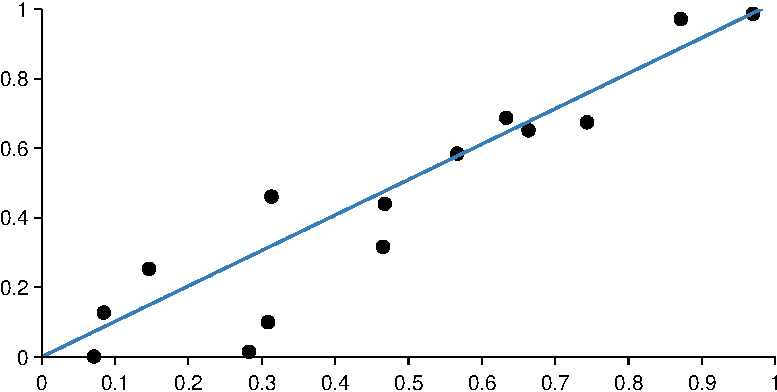
\includegraphics[width=0.8\textwidth]{figures/lin_reg/least_squares}
  \end{center}
  \begin{itemize}
    \item Common approach: Estimate $m$ by least squares
  \end{itemize}
  }
\end{frame}

\begin{frame}{How to do Bayesian linear regression} 
  \only<1>{
  \begin{center}
    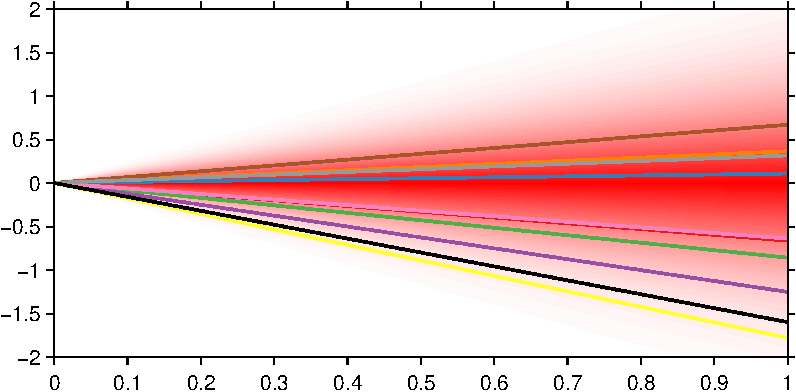
\includegraphics[width=0.8\textwidth]{figures/lin_reg/prior}
  \end{center}
  \begin{itemize}
    \item Bayesian approach:
    \begin{itemize}
      \item Specify beliefs about $m$ using probability distributions
    \end{itemize}
  \end{itemize}
  }
  \only<2>{
  \begin{center}
    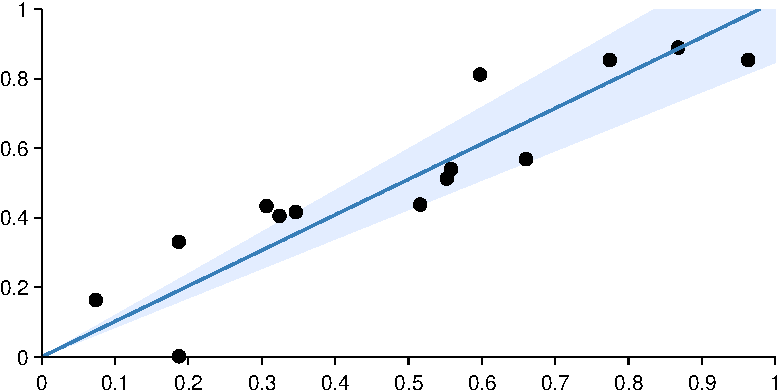
\includegraphics[width=0.8\textwidth]{figures/lin_reg/bayes_15}
  \end{center}
  \begin{itemize}
    \item Bayesian approach:
    \begin{itemize}
      \item Specify prior beliefs about $m$ using probability distributions
      \item Follow rules of probability to update beliefs rationally after observing data
    \end{itemize}
  \end{itemize}
  }
\end{frame}

\begin{frame}{Sum and product rules of probability}
  \only<1>{
  \begin{align*}
    \textrm{Sum rule :} \quad & \quad \phantom{,Y=y}\mathbb{P}(X=x) = \sum_y \mathbb{P}(X=x, Y=y) \\ \\
    \textrm{Product rule :} \quad & \quad \mathbb{P}(X=x, Y=y) = \mathbb{P}(X=x)\,\mathbb{P}(Y=y\,|\,X=x)
  \end{align*}
  }
  \only<2>{
  \begin{align*}
    \textrm{Sum rule :} \quad & \quad \phantom{,y}p(x) = \int p(x, y)\,\textrm{d}y \\ \\
    \textrm{Product rule :} \quad & \quad p(x, y) = p(x)\,p(y\,|\,x)
  \end{align*}
  }
\end{frame}

\begin{frame}{Bayesian statistics}
  \begin{itemize}
    \uncover<1->{
      \item Suppose we wish to fit a model $M$ with parameters $\theta$ to data $D$
      \begin{itemize}
        \item $M$ defined by $\textcolor{blue}{p(D\,|\,\theta,M)}$ - the likelihood
      \end{itemize}
    }
    \uncover<2->{
      \vspace{\baselineskip}
      \item We represent our uncertainty about $\theta$ with a probability distribution
      \begin{itemize}
        \item $\textcolor{red}{p(\theta\,|\,M)}$ - the prior
      \end{itemize}
    }
    \uncover<3->{
      \vspace{\baselineskip}
      \item We now derive $\textcolor{green}{p(\theta\,|\,D,M)}$ - the posterior
    }
  \end{itemize}
\end{frame}

\begin{frame}{Deriving Bayes rule}
    \uncover<1->{
      \begin{equation*}
        p(\theta, D \,|\, M) = p(\theta, D \,|\, M)
      \end{equation*}
    }
    \uncover<2->{
      \begin{equation*}
        p(\theta \,|\, D, M)p(D\,|\,M) = p(D \,|\, \theta, M)p(\theta \,|\, M) \quad \textrm{(product rule)} 
      \end{equation*}
    }
    \uncover<3->{
      \begin{equation*}
        p(\theta \,|\, D, M) = \frac{p(D \,|\, \theta, M)p(\theta \,|\, M)}{p(D\,|\,M)}
      \end{equation*}
    }
    \uncover<4->{
      \begin{equation*}
        p(\theta \,|\, D, M) = \frac{p(D \,|\, \theta, M)p(\theta \,|\, M)}{\int p(D,\theta\,|\,M)\textrm{d}\theta} \quad \textrm{(sum rule)} 
      \end{equation*}
    }
    \uncover<5>{
      \begin{equation*}
        p(\theta \,|\, D, M) = \frac{p(D \,|\, \theta, M)p(\theta \,|\, M)}{\int p(D \,|\, \theta, M)p(\theta \,|\, M)\textrm{d}\theta} \quad \textrm{(product rule)} 
      \end{equation*}
    }
\end{frame}

\begin{frame}{Bayes rule}
  \begin{itemize}
      \item Suppose we wish to fit a model $M$ with parameters $\theta$ to data $D$
      \begin{itemize}
        \item $M$ defined by $\textcolor{blue}{p(D\,|\,\theta,M)}$ - the likelihood
      \end{itemize}
      \vspace{\baselineskip}
      \item We represent our uncertainty about $\theta$ with a probability distribution
      \begin{itemize}
        \item $\textcolor{red}{p(\theta\,|\,M)}$ - the prior
      \end{itemize}
      \vspace{\baselineskip}
      \item We now derive $\textcolor{green}{p(\theta\,|\,D,M)}$ - the posterior
      \begin{equation*}
       \underbrace{\textcolor{green}{p(\theta \,|\, D, M)}}_{\textnormal{posterior}} = \frac{\overbrace{\textcolor{blue}{p(D \,|\, \theta, M)}}^{\textnormal{likelihood}}\overbrace{\textcolor{red}{p(\theta \,|\, M)}}^{\textnormal{prior}}}{\underbrace{\textcolor{purple}{\int p(D \,|\, \theta, M)p(\theta \,|\, M)\textrm{d}\theta}}_{\textnormal{marginal likelihood}}}
      \end{equation*}
  \end{itemize}
\end{frame}

\begin{frame}{Bayesian linear regression}
  \only<1>{
    \vspace{\baselineskip}
  \begin{center}
    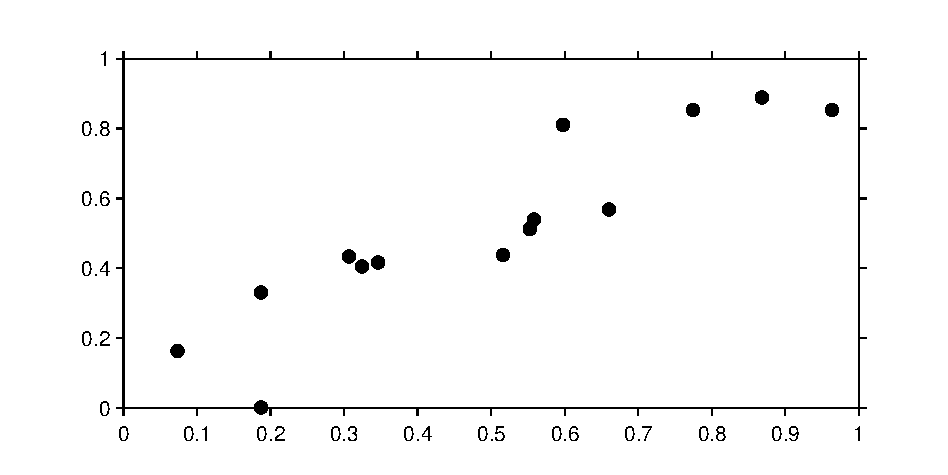
\includegraphics[width=0.8\textwidth]{figures/lin_reg/all_data}
  \end{center}
    \vspace{2\baselineskip}
  }
  \begin{itemize}
    \uncover<1->{
    \item Linear regression starts by assuming a model of the form $y_i = m x_i + \varepsilon_i$ where $x$ and $y$ are inputs and outputs respectively and $\varepsilon$ are errors or noise
    \vspace{\baselineskip}
    }
    \uncover<2->{
    \item Represent prior beliefs about $m$ using a probability distribution
    }
    \only<3>{
    \begin{itemize}
      \item \eg $m \sim \textrm{Normal}(\textrm{mean} = 0,\textrm{variance} = 1)$
    \end{itemize}
    }
    \only<4,5,6>{
    \begin{itemize}
      \item \eg $m \sim \mathcal{N}(0,1)$
    \end{itemize}
    }
    \uncover<5->{
    \vspace{\baselineskip}
    \item Define likelihood by representing prior beliefs about $\varepsilon$ using a probability distribution
    \begin{itemize}
      \item \eg $\varepsilon_i \sim \mathcal{N}(0,\sigma_\varepsilon^2)$ independently for all $i$
    \end{itemize}
    }
    \uncover<6->{
    \vspace{\baselineskip}
    \item Apply Bayes rule
    }
  \end{itemize}
\end{frame}

\begin{frame}{Bayes rule applied to linear regression}
  \vspace{-2\baselineskip}
  \begin{align*}
    p(m\,|\,y,x) = \frac{p(y\,|\,m,x)\,p(m)}{\int p(y,m,|\,x)\,\textrm{d}m}
  \end{align*}
  \pause
  \vspace{-\baselineskip}
  \begin{align*}
    p(m\,|\,y,x) \propto p(y\,|\,m,x)\,p(m)
  \end{align*}
  \vspace{-\baselineskip}
  \pause
  \begin{align*}
    p(m\,|\,y,x) \propto \bigg(\prod_i\frac{1}{2\pi\sigma_\varepsilon}e^{-(y_i-mx_i)^2/(2\sigma_\varepsilon^2)}\bigg)\frac{1}{2\pi}e^{-m^2/2}
  \end{align*}
  \vspace{-\baselineskip}
  \pause
  \begin{align*}
    p(m\,|\,y,x) \propto e^{-\sum_i(y_i-mx_i)^2/(2\sigma_\varepsilon^2) - m^2/2}
  \end{align*}
  \vspace{-\baselineskip}
  \pause
  \begin{align*}
    p(m\,|\,y,x) \propto e^{-\frac{\sum_i x_i^2 + \sigma_\varepsilon^2}{2\sigma_\varepsilon^2}\big(m - \frac{\sum_i x_i y_i}{\sum_i x_i^2 + \sigma_\varepsilon^2}\big)^2}
  \end{align*}
  \vspace{-\baselineskip}
  \pause
  This is a normal distribution $m\,|\,y,x \sim \mathcal{N}(\frac{\sum_i x_i y_i}{\sum_i x_i^2 + \sigma_\varepsilon^2}, \frac{\sigma_\varepsilon^2}{\sum_i x_i^2 + \sigma_\varepsilon^2})$
\end{frame}

\begin{frame}{Bayesian linear regression}
  \begin{center}
    \includegraphics<1>[width=0.8\textwidth]{figures/lin_reg/bayes_1}
    \includegraphics<2>[width=0.8\textwidth]{figures/lin_reg/bayes_2}
    \includegraphics<3>[width=0.8\textwidth]{figures/lin_reg/bayes_3}
    \includegraphics<4>[width=0.8\textwidth]{figures/lin_reg/bayes_5}
    \includegraphics<5>[width=0.8\textwidth]{figures/lin_reg/bayes_10}
    \includegraphics<6>[width=0.8\textwidth]{figures/lin_reg/bayes_15}
  \end{center}
  \begin{align*}
    m\,|\,y,x \sim \mathcal{N}\bigg(\frac{\sum_i x_i y_i}{\sum_i x_i^2 + \sigma_\varepsilon^2}, \frac{\sigma_\varepsilon^2}{\sum_i x_i^2 + \sigma_\varepsilon^2}\bigg)
  \end{align*}
\end{frame}

\begin{frame}{Bayesian linear regression rewritten}
  \begin{itemize}
    \item We defined a Bayesian linear regression model by specifying priors on $m$ and $\varepsilon_i$.
    \pause
    \begin{itemize}
      \item $m \sim \mathcal{N}(0, 1)$, $\varepsilon_i \simiid \mathcal{N}(0, \sigma_\varepsilon^2)$
      \pause
      \item $y_i \,|\, m, \varepsilon_i = mx_i + \varepsilon_i$
    \end{itemize}
    \vspace{\baselineskip}
    \pause
    \item This implictly defined a joint prior on $\{y_i \,:\, i=1,\ldots,n\}$
    \pause
    \begin{itemize}
      \item $y_i \sim \mathcal{N}(0, x_i^2 + \sigma_\varepsilon^2)$ (sum of two normals)
      \pause
      \item Also, $\textrm{cov}(y_i, y_j) = x_i x_j \quad \forall\,i\neq j$
    \end{itemize}
    \vspace{\baselineskip}
    \pause
    \item \ie $\{y_i \,:\, i=1,\ldots,n\}$ is jointly normally distributed
    \begin{itemize}
      \item $y \sim \mathcal{N}(\mathbf{0}, \mathbf{K})$
      \item where $k_{ij} = x_i x_j + \delta_{ij} \sigma_\varepsilon^2$
    \end{itemize}
  \end{itemize}
\end{frame}

\begin{frame}{Bayesian linear regression rewritten}
  $\{y_i \,:\, i=1,\ldots,n\}$ is jointly normally distributed
  \begin{equation*}
    y \sim \mathcal{N}(\mathbf{0}, \mathbf{K})
  \end{equation*}
  where $k_{ij} = x_i x_j + \delta_{ij} \sigma_\varepsilon^2$.
  
  \vspace{\baselineskip}
  \pause
  
  This can be written as a (kernel) function of pairs of $x_i$
  \begin{equation*}
    k_{ij} = k(x_i, x_j) = x_i x_j + \delta_{x_i = x_j}\sigma_\varepsilon^2
  \end{equation*}
  
  \vspace{\baselineskip}
  \pause
  
  Do we define a valid probability distribution if $\{x_i\} = \mathbb{R}$?
\end{frame}

\begin{frame}{Gaussian processes}
  \begin{itemize}
    \item A Gaussian process is collection of random variables, any finite number of which have a joint Gaussian distribution
    \vspace{\baselineskip}
    \item We can write this collection of random variables as $\{f(x) : x \in \mathcal{X}\}$ \ie a function $f$ evaluated at inputs $x$
    \vspace{\baselineskip}
    \item A \gp{} is completely specified by
    \begin{itemize}
      \item Mean function, $\mu(x)=\mathbb{E}(f(x))$
      \item Covariance / kernel function, $\kernel(x,x') = \Cov(f(x),f(x'))$
      \item Denoted $f \,\sim\, \gp{}(\mu,\kernel)$
    \end{itemize}
    \vspace{\baselineskip}
    \item Can be thought of as a probability distribution on functions
  \end{itemize}
\end{frame}

\begin{frame}{Linear kernel = linear functions}
  \begin{center}
    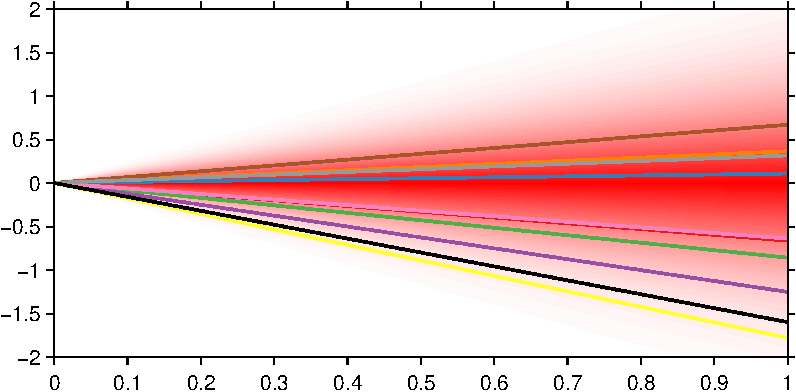
\includegraphics[width=0.8\textwidth]{figures/lin_reg/prior}
  \end{center}
  \begin{equation*}
    k(x, x') = xx'
  \end{equation*}
\end{frame}

\begin{frame}{What about other kernels?}
  \begin{center}
    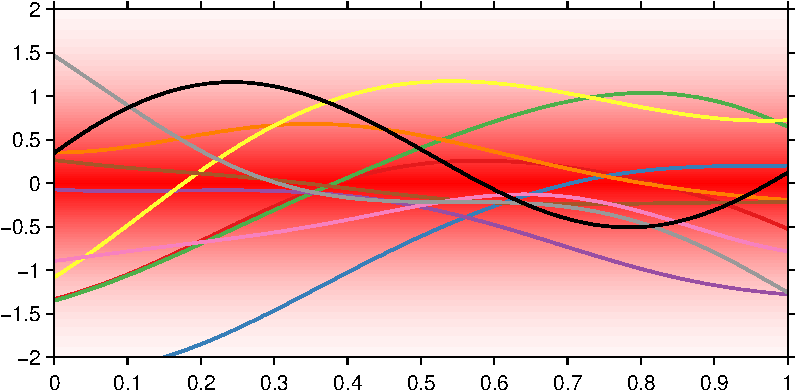
\includegraphics[width=0.8\textwidth]{figures/lin_reg/sq_exp_prior}
  \end{center}
  \begin{equation*}
    k(x, x') = e^{-(x-x')^2}
  \end{equation*}
\end{frame}

\begin{frame}{Bayesian non-linear regression}
  \begin{center}
    \includegraphics<1>[width=0.8\textwidth]{figures/lin_reg/sq_exp_1}
    \includegraphics<2>[width=0.8\textwidth]{figures/lin_reg/sq_exp_2}
    \includegraphics<3>[width=0.8\textwidth]{figures/lin_reg/sq_exp_3}
    \includegraphics<4>[width=0.8\textwidth]{figures/lin_reg/sq_exp_5}
    \includegraphics<5>[width=0.8\textwidth]{figures/lin_reg/sq_exp_10}
    \includegraphics<6>[width=0.8\textwidth]{figures/lin_reg/sq_exp_15}
  \end{center}
\end{frame}

\begin{frame}{Bayesian linear regression gone wrong}
  \begin{center}
    \includegraphics<1>[width=0.8\textwidth]{figures/quad/bayes_1}
    \includegraphics<2>[width=0.8\textwidth]{figures/quad/bayes_2}
    \includegraphics<3>[width=0.8\textwidth]{figures/quad/bayes_3}
    \includegraphics<4>[width=0.8\textwidth]{figures/quad/bayes_5}
    \includegraphics<5>[width=0.8\textwidth]{figures/quad/bayes_10}
    \includegraphics<6>[width=0.8\textwidth]{figures/quad/bayes_15}
  \end{center}
\end{frame}

\begin{frame}{Non-linearity to the rescue}
  \begin{center}
    \includegraphics<1>[width=0.8\textwidth]{figures/quad/sq_exp_1}
    \includegraphics<2>[width=0.8\textwidth]{figures/quad/sq_exp_2}
    \includegraphics<3>[width=0.8\textwidth]{figures/quad/sq_exp_3}
    \includegraphics<4>[width=0.8\textwidth]{figures/quad/sq_exp_5}
    \includegraphics<5>[width=0.8\textwidth]{figures/quad/sq_exp_10}
    \includegraphics<6>[width=0.8\textwidth]{figures/quad/sq_exp_15}
  \end{center}
\end{frame}

\begin{frame}{Which kernel function?}
  How far can we go with kernel functions?
\end{frame}

\begin{frame}{Defining a language of models}
    % Define block styles
  \tikzstyle{block} = [rectangle, draw, fill=blue!20, 
                       text width=4.4em, text centered, rounded corners, minimum height=3em]
  \tikzstyle{line} = [draw, -latex']
  \tikzstyle{cloud} = [draw, ellipse,fill=red!20,minimum height=2em]
  \tikzstyle{supercloud} = [draw, ellipse,fill=red!50,minimum height=2em,]
    
  \begin{tikzpicture}[node distance = 2.3cm]
    \footnotesize
    % Place nodes
    \node [cloud] (data) {Data};
    \node [block, right of=data] (search) {Search};
    \node [supercloud, above of=search] (language) {\bf Language of models};
    \node [block, below of=search] (eval) {Evaluation};
    \node [cloud, right of=search] (model) {Model};
    \node [block, right of=model] (pred) {Prediction};
    \node [block, above of=pred] (trans) {Description};
    \node [block, below of=pred] (checking) {Checking};
    \node [cloud, right of=pred] (report) {Report};
    % Draw edges
    \path [line] (data) -- (search);
    \path [line] (language) -- (search);
    \path [line] (search) -- (model);
    \path [line] (search) -- (model);
    \path [line] (model.north east) -- (trans.south west);
    \path [line] (model.east) -- (pred.west);
    \path [line] (model.south east) -- (checking.north west);
    \path [line] (trans.south east) -- (report.north west);
    \path [line] (pred.east) -- (report.west);
    \path [line] (checking.north east) -- (report.south west);
    \draw[->,] (search.south east) .. controls (3.45,-1.15) .. (eval.north east);
    \draw[->,] (eval.north west) .. controls (1.15,-1.15) .. (search.south west);
  \end{tikzpicture}
\end{frame}

\begin{frame}{The atoms of our language}  
  \newcommand{\fhbig}{1.0cm}
\newcommand{\fwbig}{1.2cm}
\newcommand{\kernpic}[1]{\includegraphics[height=\fhbig,width=\fwbig]{../figures/structure_examples/#1}}
\newcommand{\colsize}{1.7cm}
\newcommand{\sepsize}{0.0cm}

Five base kernels\dots

\vspace{\baselineskip}

\begin{tabularx}{\columnwidth}{x{\colsize}x{\colsize}x{\colsize}x{\colsize}x{\colsize}}
  \kernpic{se_kernel} & \kernpic{per_kernel} & \kernpic{lin_kernel} & \kernpic{c_kernel} & \kernpic{wn_kernel} \\
  {\footnotesize Squared \newline exp. (\kSE)} & {\footnotesize Periodic (\kPer)} & {\footnotesize Linear (\kLin)} & {\footnotesize Constant (\kC)} & {\footnotesize White \newline noise (\kWN)}
\end{tabularx}

\vspace{\baselineskip}

\dots encoding for the following types of functions

\vspace{\baselineskip}

\begin{tabularx}{\columnwidth}{x{\colsize}x{\colsize}x{\colsize}x{\colsize}x{\colsize}}
  \kernpic{se_kernel_draws} & \kernpic{per_kernel_draws_s2} & \kernpic{lin_kernel_draws} & \kernpic{c_kernel_draws} & \kernpic{wn_kernel_draws} \\
  {\footnotesize Smooth \newline functions} & {\footnotesize Periodic functions} & {\footnotesize Linear \newline functions} & {\footnotesize Constant \newline functions} & {\footnotesize Gaussian \newline noise} 
\end{tabularx}


\end{frame}

\begin{frame}{The composition rules of our language}
\begin{itemize} 
	\item Two main operations: addition, multiplication
\end{itemize}
\newcommand{\fhbig}{1.6cm}
\newcommand{\fwbig}{1.8cm}
\newcommand{\kernpic}[1]{\includegraphics[height=\fhbig,width=\fwbig]{figures/structure_examples/#1}}
\newcommand{\largeplus}{\tabbox{{\Large+}}}
\newcommand{\largeeq}{\tabbox{{\Large=}}}
\newcommand{\largetimes}{\tabbox{{\Large$\times$}}}
\begin{figure}[ht]
\centering
\renewcommand{\tabularxcolumn}[1]{>{\arraybackslash}m{#1}}
\begin{tabularx}{\columnwidth}{XXcXX}
  {\small $\kLin \times \kLin$} & \kernpic{lin_times_lin_draws} & \phantom{mm}
& {\small $\kSE \times \kPer$} & \kernpic{longse_times_per_draws_s1}
\\
   & {\small quadratic functions} & \phantom{mm}
&  & {\small locally \newline periodic}
\\ \\
%\midrule 
  {\small $\kLin + \kPer$} & \kernpic{lin_plus_per_draws} & \phantom{mm} 
& {\small $\kSE + \kPer$ } & \kernpic{se_plus_per_draws_s7}
\\
   & {\small periodic plus linear trend} & \phantom{mm}
&  & {\small periodic plus smooth trend}
\end{tabularx}
\end{figure}


\end{frame}

\begin{frame}{An expressive language of models}
\begin{center}
\begin{tabular}{l|l}
Regression model & Kernel \\
\midrule
\gp{} smoothing & $\kSE + \kWN$ \\
Linear regression & $\kC + \kLin + \kWN$ \\
Multiple kernel learning & $\sum \kSE$ + \kWN\\
Trend, cyclical, irregular & $\sum \kSE + \sum \kPer$ + \kWN\\
Fourier decomposition & $\kC + \sum \cos$ + \kWN\\
Sparse spectrum \gp{}s & $\sum \cos$ + \kWN\\
Spectral mixture & $\sum \SE \times \cos$ + \kWN\\
Heteroscedasticity & \eg $\kSE + \kLin \times \kWN$
\end{tabular}
\end{center}
Note: $\cos$ is a special case of our version of $\kPer$
\end{frame}

\begin{frame}{Discovering a good model via search}
    % Define block styles
  \tikzstyle{block} = [rectangle, draw, fill=blue!20, 
                       text width=4.4em, text centered, rounded corners, minimum height=3em]
  \tikzstyle{superblock} = [rectangle, draw, fill=blue!50, 
                       text width=4.4em, text centered, rounded corners, minimum height=3em]
  \tikzstyle{line} = [draw, -latex']
  \tikzstyle{cloud} = [draw, ellipse,fill=red!20,minimum height=2em]
  \tikzstyle{supercloud} = [draw, ellipse,fill=red!50,minimum height=2em]
    
  \begin{tikzpicture}[node distance = 2.3cm]
    \footnotesize
    % Place nodes
    \node [cloud] (data) {Data};
    \node [superblock, right of=data] (search) {\bf Search};
    \node [cloud, above of=search] (language) {Language};
    \node [block, below of=search] (eval) {Evaluation};
    \node [cloud, right of=search] (model) {Model};
    \node [block, right of=model] (pred) {Prediction};
    \node [block, above of=pred] (trans) {Translation};
    \node [block, below of=pred] (checking) {Checking};
    \node [cloud, right of=pred] (report) {Report};
    % Draw edges
    \path [line] (data) -- (search);
    \path [line] (language) -- (search);
    \path [line] (search) -- (model);
    \path [line] (search) -- (model);
    \path [line] (model.north east) -- (trans.south west);
    \path [line] (model.east) -- (pred.west);
    \path [line] (model.south east) -- (checking.north west);
    \path [line] (trans.south east) -- (report.north west);
    \path [line] (pred.east) -- (report.west);
    \path [line] (checking.north east) -- (report.south west);
    \draw[->,] (search.south east) .. controls (3.45,-1.15) .. (eval.north east);
    \draw[->,] (eval.north west) .. controls (1.15,-1.15) .. (search.south west);
  \end{tikzpicture}
\end{frame}

\begin{frame}{Discovering a good model via search}
  \begin{itemize}
    \item Language defined as the arbitrary composition of five base kernels ($\kWN, \kC, \kLin, \kSE, \kPer$) via two operators ($+, \times$). 
    \vspace{\baselineskip}
    \item The space spanned by this language is open-ended and can have a high branching factor requiring a judicious search
    \vspace{\baselineskip}
    \item We propose a greedy search for its simplicity and similarity to human model-building
  \end{itemize}
\end{frame}

\begin{frame}{Example: Mauna Loa Keeling Curve}
\hspace{-1.2cm}
\only<1>{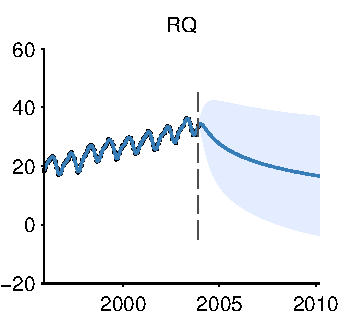
\includegraphics[width=0.4\textwidth]{figures/11-Feb-v4-03-mauna2003-s_max_level_0/03-mauna2003-s_all_small.pdf}}
\only<2>{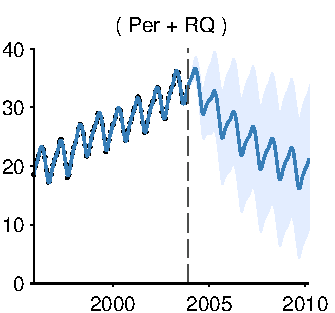
\includegraphics[width=0.4\textwidth]{figures/11-Feb-v4-03-mauna2003-s_max_level_1/03-mauna2003-s_all_small.pdf}}
\only<3>{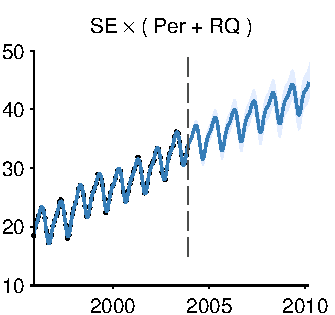
\includegraphics[width=0.4\textwidth]{figures/11-Feb-v4-03-mauna2003-s_max_level_2/03-mauna2003-s_all_small.pdf}}
\only<4>{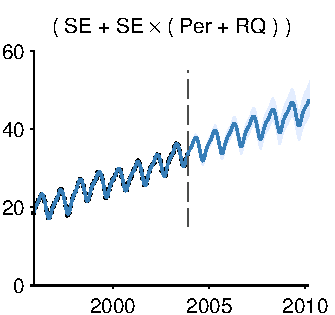
\includegraphics[width=0.4\textwidth]{figures/11-Feb-v4-03-mauna2003-s_max_level_3/03-mauna2003-s_all_small.pdf}}

\vspace{-3.5cm}
\begin{minipage}[t][14cm][t]{1.14\linewidth}
\begin{flushleft}
\hspace{5.5cm}
\vspace{-8cm}
\makebox[\textwidth][c]{
\raisebox{10cm}{
\vspace{-8cm}
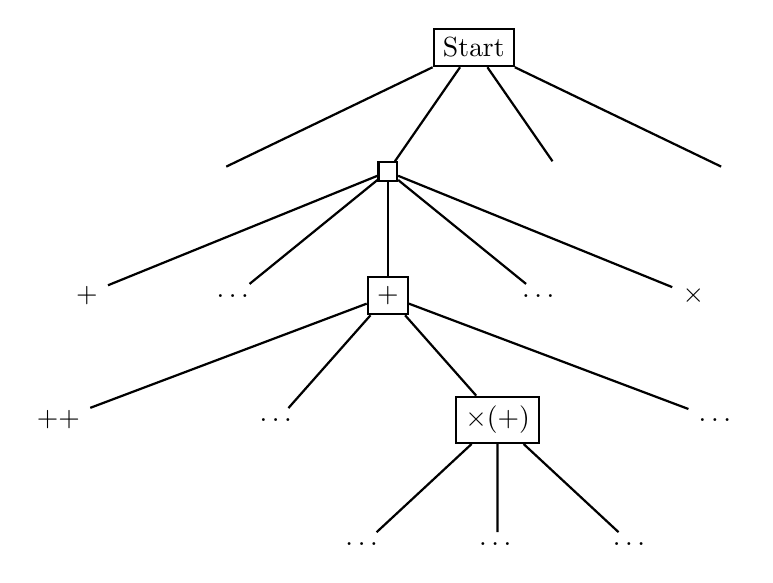
\begin{tikzpicture}
[sibling distance=0.18\columnwidth,-,thick, level distance=0.13\columnwidth]
%\footnotesize
\node[shape=rectangle,draw,thick] {Start}
%\pause
  child {node {$\SE$}}
%  fill=camlightblue!30
  child {node[shape=rectangle,draw,thick] {$\RQ$}
    [sibling distance=0.16\columnwidth]
%    {\visible<2->{ child {node {\ldots}}}}
    child [hide on=-1] {node {$\SE$ + \RQ}}
    child [hide on=-1] {node {\ldots}}
    child [hide on=-1] {node[shape=rectangle,draw,thick] {$\Per + \RQ$}
      [sibling distance=0.23\columnwidth]
      child [hide on=-2] {node {$\SE + \Per + \RQ$}}
      child [hide on=-2] {node {\ldots}}
      child [hide on=-2] {node[shape=rectangle,draw,thick] {$\SE \times (\Per + \RQ)$}
        [sibling distance=0.14\columnwidth]
        child [hide on=-3] {node {\ldots}}
        child [hide on=-3] {node {\ldots}}
        child [hide on=-3] {node {\ldots}}
      }
      child [hide on=-2] {node {\ldots}}
    }
    %child {node {$\RQ \times \SE$}}
    child [hide on=-1] {node {\ldots}}
    child [hide on=-1] {node {$\Per \times \RQ$}}
  }
  child {node {$\Lin$}}
  child {node {$\Per$}}
  ;
\end{tikzpicture}}
}\end{flushleft}
\end{minipage}
\only<4>{}
\end{frame}

\begin{frame}{Model evaluation}
    % Define block styles
  \tikzstyle{block} = [rectangle, draw, fill=blue!20, 
                       text width=4.4em, text centered, rounded corners, minimum height=3em]
  \tikzstyle{superblock} = [rectangle, draw, fill=blue!50, 
                       text width=4.4em, text centered, rounded corners, minimum height=3em]
  \tikzstyle{line} = [draw, -latex']
  \tikzstyle{cloud} = [draw, ellipse,fill=red!20,minimum height=2em]
  \tikzstyle{supercloud} = [draw, ellipse,fill=red!50,minimum height=2em]
    
  \begin{tikzpicture}[node distance = 2.3cm]
    \footnotesize
    % Place nodes
    \node [cloud] (data) {Data};
    \node [block, right of=data] (search) {Search};
    \node [cloud, above of=search] (language) {Language of models};
    \node [superblock, below of=search] (eval) {\bf Evaluation};
    \node [cloud, right of=search] (model) {Model};
    \node [block, right of=model] (pred) {Prediction};
    \node [block, above of=pred] (trans) {Description};
    \node [block, below of=pred] (checking) {Checking};
    \node [cloud, right of=pred] (report) {Report};
    % Draw edges
    \path [line] (data) -- (search);
    \path [line] (language) -- (search);
    \path [line] (search) -- (model);
    \path [line] (search) -- (model);
    \path [line] (model.north east) -- (trans.south west);
    \path [line] (model.east) -- (pred.west);
    \path [line] (model.south east) -- (checking.north west);
    \path [line] (trans.south east) -- (report.north west);
    \path [line] (pred.east) -- (report.west);
    \path [line] (checking.north east) -- (report.south west);
    \draw[->,] (search.south east) .. controls (3.45,-1.15) .. (eval.north east);
    \draw[->,] (eval.north west) .. controls (1.15,-1.15) .. (search.south west);
  \end{tikzpicture}
\end{frame}

\begin{frame}{Bayesian model selection}
  \uncover<1->{
    Suppose we have a collection of models $\{M_i\}$ and some data $D$
    
    \vspace{\baselineskip}
    
  }
  \uncover<2->{
    Bayes rule tells us
    \begin{equation*}
      p(M_i\,|\,D) = \frac{p(D\,|\,M_i)p(M_i)}{p(D)}
    \end{equation*}
  }
  \uncover<3->{
    If $p(M_i)$ is equal for all $i$ (prior ignorance) then
    \begin{equation*}
      p(M_i\,|\,D) \propto p(D\,|\,M_i) = \int p(D\,|\,\theta_i,M_i)p(\theta_i\,|\,M_i)\textrm{d}\theta_i
    \end{equation*}
  }
  \uncover<4->{
    \ie The most likely model has the highest \textcolor{purple}{marginal likelihood}
  }
\end{frame}

\begin{frame}{Automatic translation of models}
    % Define block styles
  \tikzstyle{block} = [rectangle, draw, fill=blue!20, 
                       text width=4.4em, text centered, rounded corners, minimum height=3em]
  \tikzstyle{superblock} = [rectangle, draw, fill=blue!50, 
                       text width=4.4em, text centered, rounded corners, minimum height=3em]
  \tikzstyle{line} = [draw, -latex']
  \tikzstyle{cloud} = [draw, ellipse,fill=red!20,minimum height=2em]
  \tikzstyle{supercloud} = [draw, ellipse,fill=red!50,minimum height=2em]
    
  \begin{tikzpicture}[node distance = 2.3cm]
    \footnotesize
    % Place nodes
    \node [cloud] (data) {Data};
    \node [block, right of=data] (search) {Search};
    \node [cloud, above of=search] (language) {Language of models};
    \node [block, below of=search] (eval) {Evaluation};
    \node [cloud, right of=search] (model) {Model};
    \node [block, right of=model] (pred) {Prediction};
    \node [superblock, above of=pred] (trans) {Translation};
    \node [block, below of=pred] (checking) {Checking};
    \node [cloud, right of=pred] (report) {Report};
    % Draw edges
    \path [line] (data) -- (search);
    \path [line] (language) -- (search);
    \path [line] (search) -- (model);
    \path [line] (search) -- (model);
    \path [line] (model.north east) -- (trans.south west);
    \path [line] (model.east) -- (pred.west);
    \path [line] (model.south east) -- (checking.north west);
    \path [line] (trans.south east) -- (report.north west);
    \path [line] (pred.east) -- (report.west);
    \path [line] (checking.north east) -- (report.south west);
    \draw[->,] (search.south east) .. controls (3.45,-1.15) .. (eval.north east);
    \draw[->,] (eval.north west) .. controls (1.15,-1.15) .. (search.south west);
  \end{tikzpicture}
\end{frame}

\begin{frame}{Automatic translation of models}
  \begin{itemize}
    \item Search can produce {\bf arbitrarily complicated models} from open-ended language but two main properties allow description to be automated
    \vspace{\baselineskip}
    \item Kernels can be {\bf decomposed} into a {\bf sum of products}
    \begin{itemize}
      \item A sum of kernels corresponds to a sum of functions
      \item Therefore, we can describe each product of kernels separately
    \end{itemize}
    \vspace{\baselineskip}
    \item Each kernel in a product modifies a model in a {\bf consistent} way
    \begin{itemize}
      \item Each kernel roughly corresponds to an adjective
    \end{itemize}
  \end{itemize}
\end{frame}

\begin{frame}{Sum of products normal form}
  Suppose the search finds the following kernel
  \begin{align*}
    \kSE \times (\kWN \times \kLin + \kC + \kPer)
  \end{align*}
  \pause
  Multiplication can be distributed over addition
  \begin{align*}
    \kSE \times \kWN \times \kLin + \kSE \times \kC + \kSE \times \kPer
  \end{align*}
  \pause
  Simplification rules are applied
  \begin{align*}
    \kWN \times \kLin + \kSE + \kSE \times \kPer
  \end{align*}
\end{frame}

\begin{frame}{Sums of kernels are sums of functions}
  If ${\textcolor{red}{f_1} \,\sim\, \gp{}(0, \textcolor{red}{\kernel_1})}$ and independently ${\textcolor{blue}{f_2} \,\sim\, \gp{}(0, \textcolor{blue}{\kernel_2})}$ then
  \begin{align*}
  \textcolor{red}{f_1} + \textcolor{blue}{f_2} \,\sim\, \gp{}(0, \textcolor{red}{\kernel_1} + \textcolor{blue}{\kernel_2})
  \end{align*}
  
\eg

\vspace{\baselineskip}

\begin{tabular}{ccccccc}
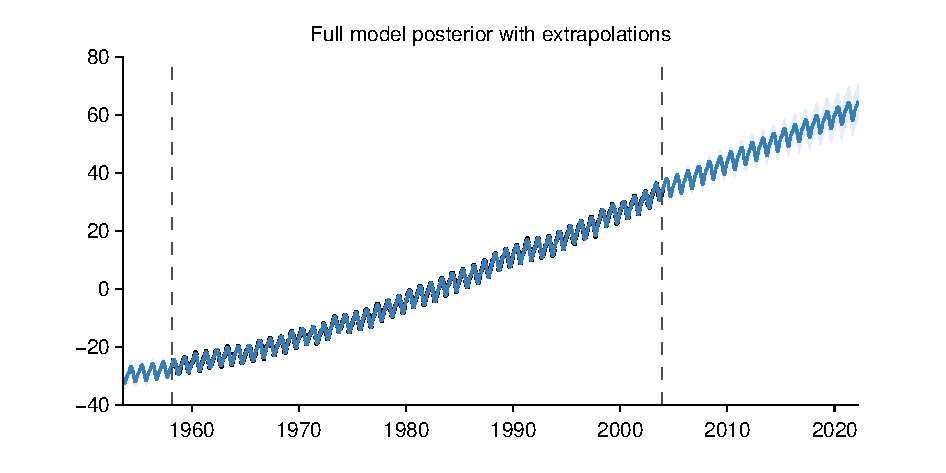
\includegraphics[trim=30 0 62 25, clip, width=0.15\textwidth]{figures/03-mauna2003_all} &
\raisebox{0.4cm}{$=$} &
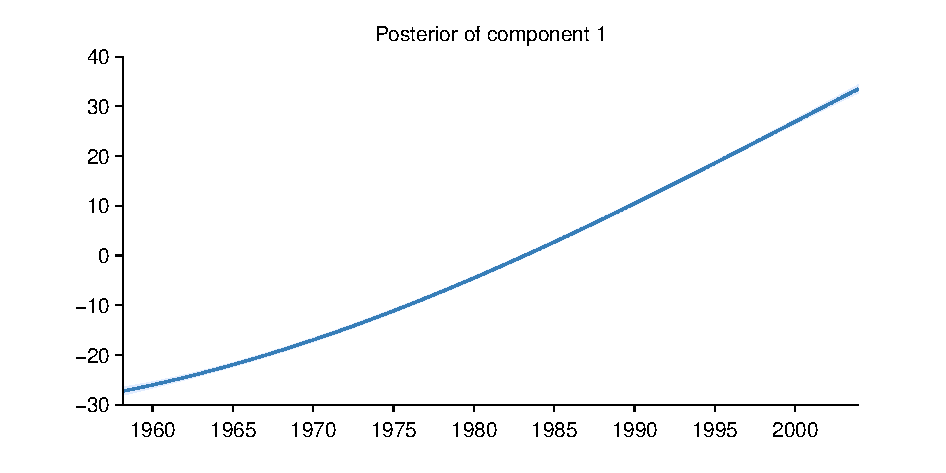
\includegraphics[trim=30 0 62 25, clip, width=0.15\textwidth]{figures/03-mauna2003_1} &
\raisebox{0.4cm}{$+$} &
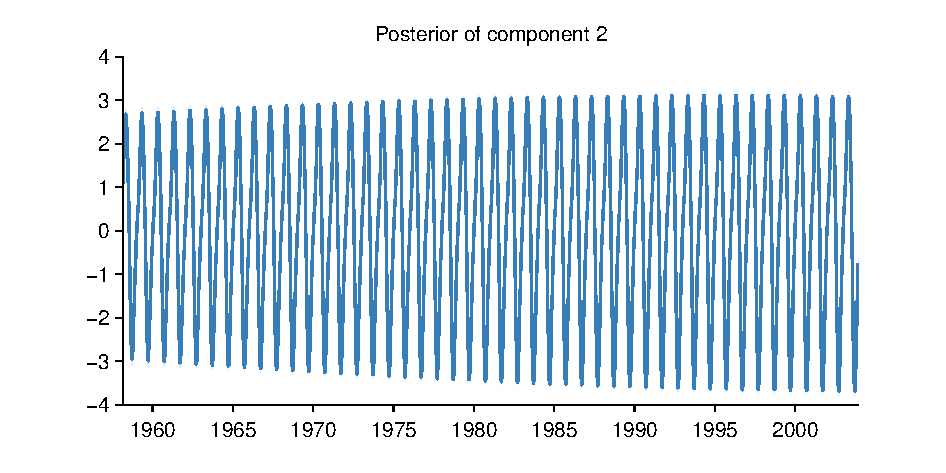
\includegraphics[trim=30 0 62 25, clip, width=0.15\textwidth]{figures/03-mauna2003_2} &
\raisebox{0.4cm}{$+$} &
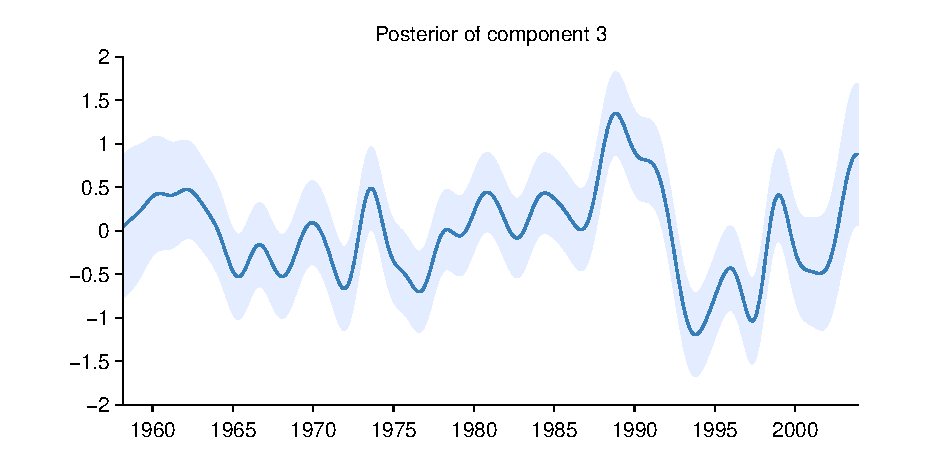
\includegraphics[trim=30 0 62 25, clip, width=0.15\textwidth]{figures/03-mauna2003_3}
\end{tabular}

\vspace{\baselineskip}

\begin{tabular}{ccccccc}
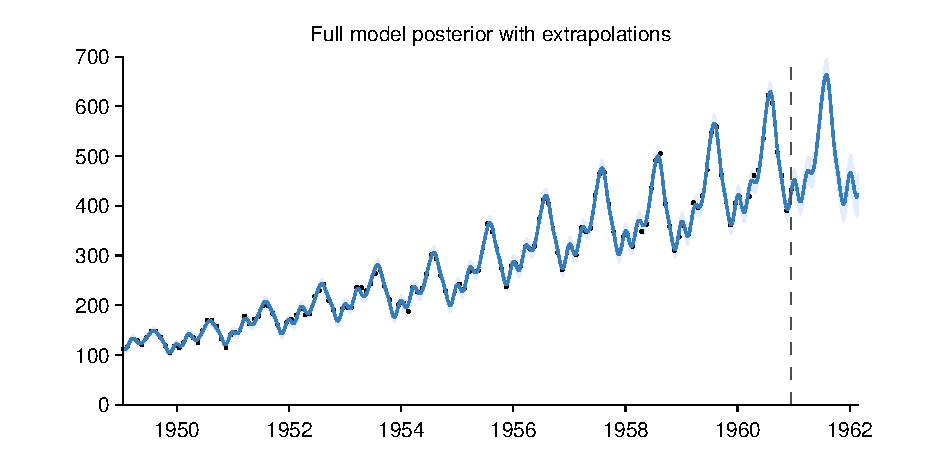
\includegraphics[trim=30 0 62 25, clip, width=0.15\textwidth]{figures/01-airline_all} &
\raisebox{0.4cm}{$=$} &
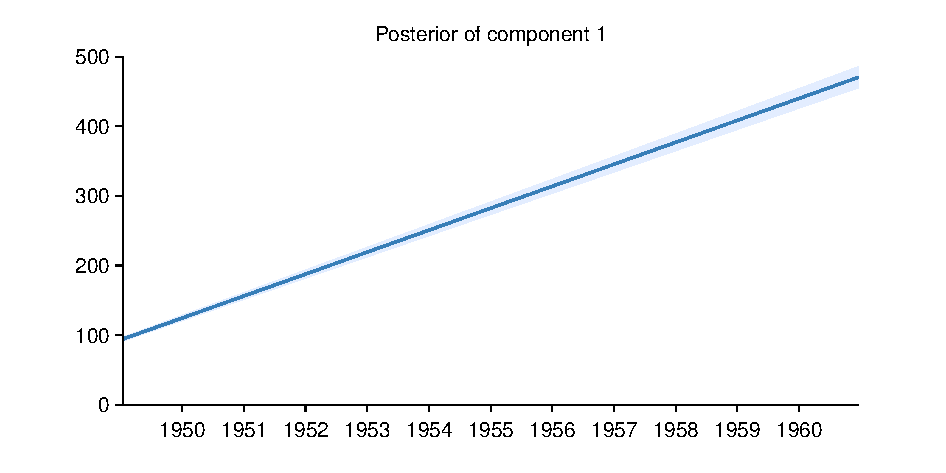
\includegraphics[trim=30 0 62 25, clip, width=0.15\textwidth]{figures/01-airline_1} &
\raisebox{0.4cm}{$+$} &
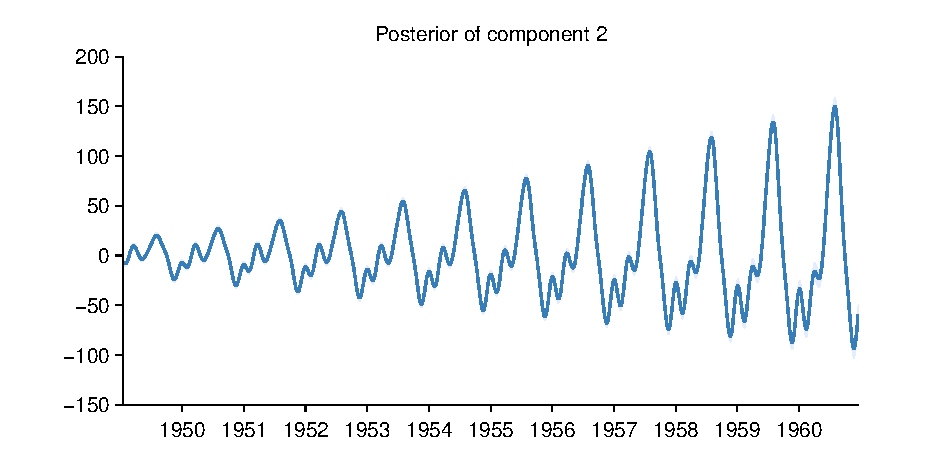
\includegraphics[trim=30 0 62 25, clip, width=0.15\textwidth]{figures/01-airline_2} &
\raisebox{0.4cm}{$+$} &
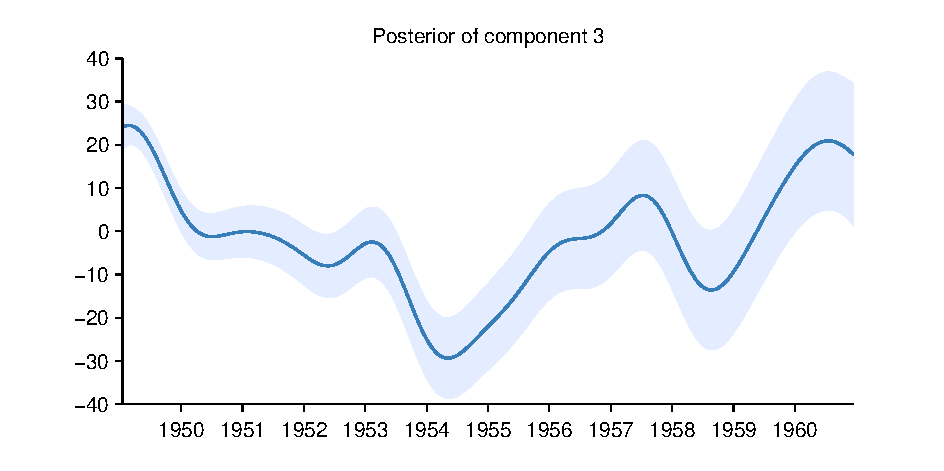
\includegraphics[trim=30 0 62 25, clip, width=0.15\textwidth]{figures/01-airline_3}
\end{tabular}

\vspace{\baselineskip}

We can therefore describe each component separately

\end{frame}

\begin{frame}{Products of kernels}
  \begin{align*}
    \phantom{\underbrace{\kSE}_{\textnormal{\scriptsize approximately}} \times }
    \underbrace{\kPer}_{\textnormal{\scriptsize periodic function}} \phantom{\times 
    \underbrace{\kLin}_{\textnormal{\scriptsize with linearly growing amplitude}}}
  \end{align*}
  
  \vspace{\baselineskip}
  
  On their own, each kernel is described by a standard noun phrase
  
  \vspace{\baselineskip}
  
  \begin{block}{}
    \begin{tabular}{cccc}
      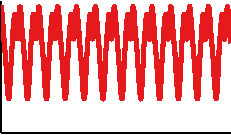
\includegraphics[width=0.2\textwidth]{figures/trans_samples/draw_11} &
      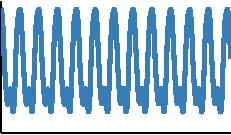
\includegraphics[width=0.2\textwidth]{figures/trans_samples/draw_12} &
      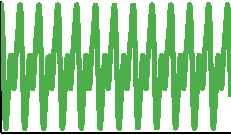
\includegraphics[width=0.2\textwidth]{figures/trans_samples/draw_13} &
      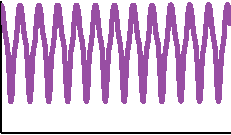
\includegraphics[width=0.2\textwidth]{figures/trans_samples/draw_14}
    \end{tabular}
  \end{block}
\end{frame}

\begin{frame}{Products of kernels - $\kSE$}
  \begin{align*}
    \underbrace{\kSE}_{\textnormal{\scriptsize approximately}} \times
    \underbrace{\kPer}_{\textnormal{\scriptsize periodic function}} \phantom{\times 
    \underbrace{\kLin}_{\textnormal{\scriptsize with linearly growing amplitude}}}
  \end{align*}
  
  \vspace{\baselineskip}
  
  {\bf Multiplication by $\kSE$} removes long range correlations from a model since $\kSE(x,x')$ decreases monotonically to 0 as $|x - x'|$ increases.
  
  \vspace{\baselineskip}
  
  \begin{block}{}
    \begin{tabular}{cccc}
      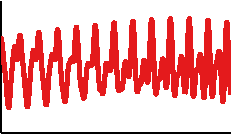
\includegraphics[width=0.2\textwidth]{figures/trans_samples/draw_21} &
      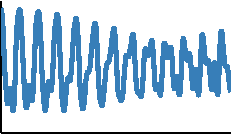
\includegraphics[width=0.2\textwidth]{figures/trans_samples/draw_22} &
      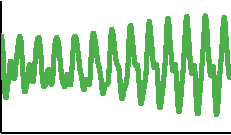
\includegraphics[width=0.2\textwidth]{figures/trans_samples/draw_23} &
      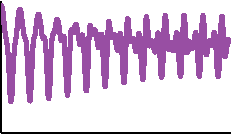
\includegraphics[width=0.2\textwidth]{figures/trans_samples/draw_24}
    \end{tabular}
  \end{block}
\end{frame}

\begin{frame}{Products of kernels - $\kLin$}
  \begin{align*}
    \underbrace{\kSE}_{\textnormal{\scriptsize approximately}} \times
    \underbrace{\kPer}_{\textnormal{\scriptsize periodic function}} \times 
    \underbrace{\kLin}_{\textnormal{\scriptsize with linearly growing amplitude}}
  \end{align*}
  
  \vspace{\baselineskip}
  
  {\bf Multiplication by $\kLin$} is equivalent to multiplying the function being modeled by a linear function.
If $f(x) \,\sim\, \gp{}(0, \kernel)$, then $x\,f(x) \,\sim\, \gp{}\left(0, k \times \kLin \right)$.
This causes the standard deviation of the model to vary linearly without affecting the correlation.
  
  \vspace{\baselineskip}
  
  \begin{block}{}
    \begin{tabular}{cccc}
      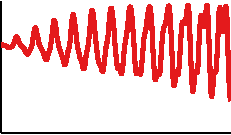
\includegraphics[width=0.2\textwidth]{figures/trans_samples/draw_31} &
      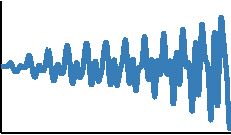
\includegraphics[width=0.2\textwidth]{figures/trans_samples/draw_32} &
      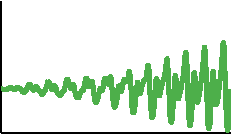
\includegraphics[width=0.2\textwidth]{figures/trans_samples/draw_33} &
      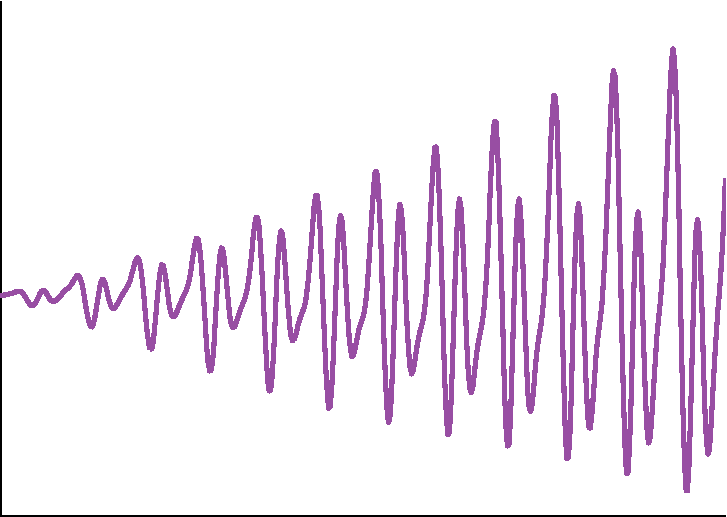
\includegraphics[width=0.2\textwidth]{figures/trans_samples/draw_34}
    \end{tabular}
  \end{block}
\end{frame}

\begin{frame}{Automatically generated reports}
    % Define block styles
  \tikzstyle{block} = [rectangle, draw, fill=blue!20, 
                       text width=4.4em, text centered, rounded corners, minimum height=3em]
  \tikzstyle{superblock} = [rectangle, draw, fill=blue!50, 
                       text width=4.4em, text centered, rounded corners, minimum height=3em]
  \tikzstyle{line} = [draw, -latex']
  \tikzstyle{cloud} = [draw, ellipse,fill=red!20,minimum height=2em]
  \tikzstyle{supercloud} = [draw, ellipse,fill=red!50,minimum height=2em]
    
  \begin{tikzpicture}[node distance = 2.3cm]
    \footnotesize
    % Place nodes
    \node [cloud] (data) {Data};
    \node [block, right of=data] (search) {Search};
    \node [cloud, above of=search] (language) {Language of models};
    \node [block, below of=search] (eval) {Evaluation};
    \node [cloud, right of=search] (model) {Model};
    \node [block, right of=model] (pred) {Prediction};
    \node [block, above of=pred] (trans) {Description};
    \node [block, below of=pred] (checking) {Checking};
    \node [supercloud, right of=pred] (report) {\bf Report};
    % Draw edges
    \path [line] (data) -- (search);
    \path [line] (language) -- (search);
    \path [line] (search) -- (model);
    \path [line] (search) -- (model);
    \path [line] (model.north east) -- (trans.south west);
    \path [line] (model.east) -- (pred.west);
    \path [line] (model.south east) -- (checking.north west);
    \path [line] (trans.south east) -- (report.north west);
    \path [line] (pred.east) -- (report.west);
    \path [line] (checking.north east) -- (report.south west);
    \draw[->,] (search.south east) .. controls (3.45,-1.15) .. (eval.north east);
    \draw[->,] (eval.north west) .. controls (1.15,-1.15) .. (search.south west);
  \end{tikzpicture}
\end{frame}

\begin{frame}{Example: Airline passenger volume}
\newcommand{\wmgd}{0.5\columnwidth}
\newcommand{\hmgd}{3.0cm}
\newcommand{\mdrd}{figures/01-airline}
\newcommand{\mbm}{\hspace{-0.3cm}}
\begin{tabular}{cc}
\mbm 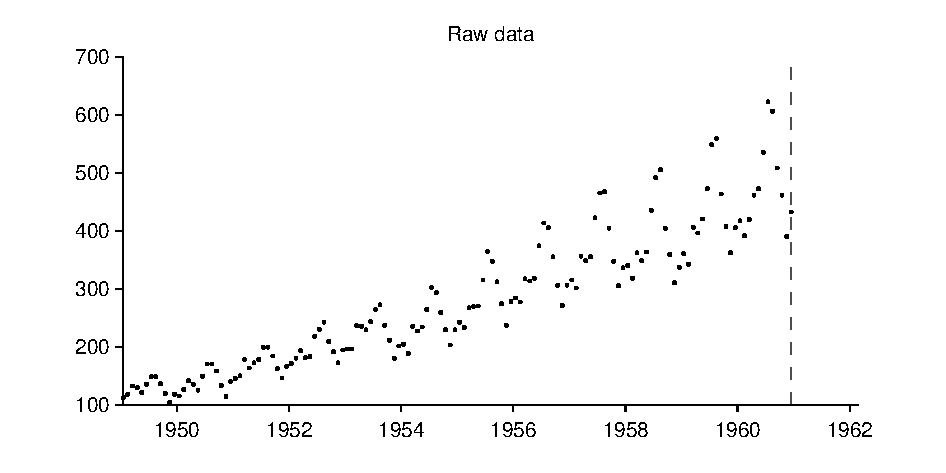
\includegraphics[width=\wmgd,height=\hmgd]{\mdrd/01-airline_raw_data} & 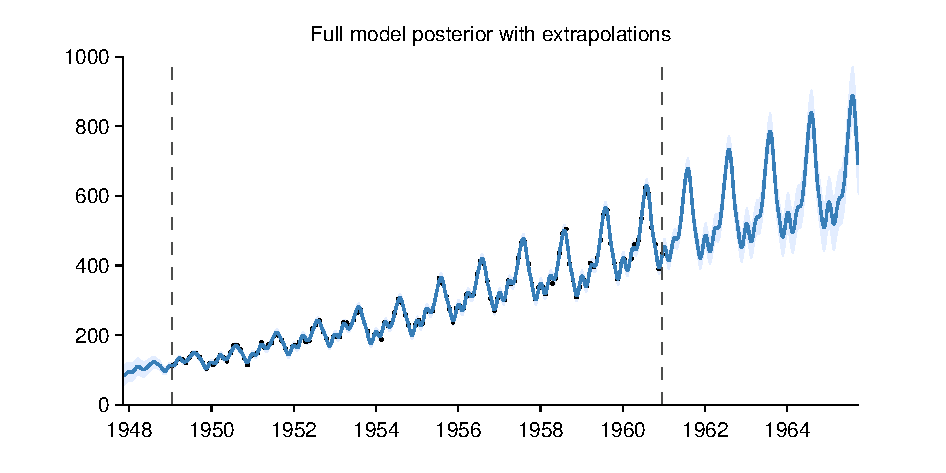
\includegraphics[width=\wmgd,height=\hmgd]{\mdrd/01-airline_all}
\end{tabular}

{\footnotesize
Four additive components have been identified in the data
\begin{itemize}

  \item A linearly increasing function. 

  \item An approximately periodic function with a period of 1.0 years and with linearly increasing amplitude. 

  \item A smooth function. 

  \item Uncorrelated noise with linearly increasing standard deviation. 

\end{itemize}
}
\end{frame}

\begin{frame}{Example: Airline passenger volume}
\newcommand{\wmgd}{0.5\columnwidth}
\newcommand{\hmgd}{3.0cm}
\newcommand{\mdrd}{figures/01-airline}
\newcommand{\mbm}{\hspace{-0.3cm}}
{\footnotesize
This function is very smooth and monotonically increasing.
}

\vspace{\baselineskip}

\begin{tabular}{cc}
\mbm 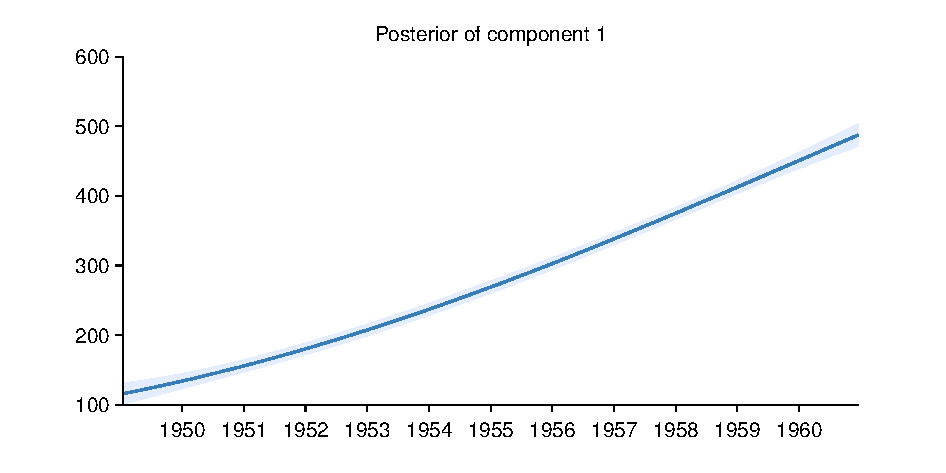
\includegraphics[width=\wmgd,height=\hmgd]{\mdrd/01-airline_1} & 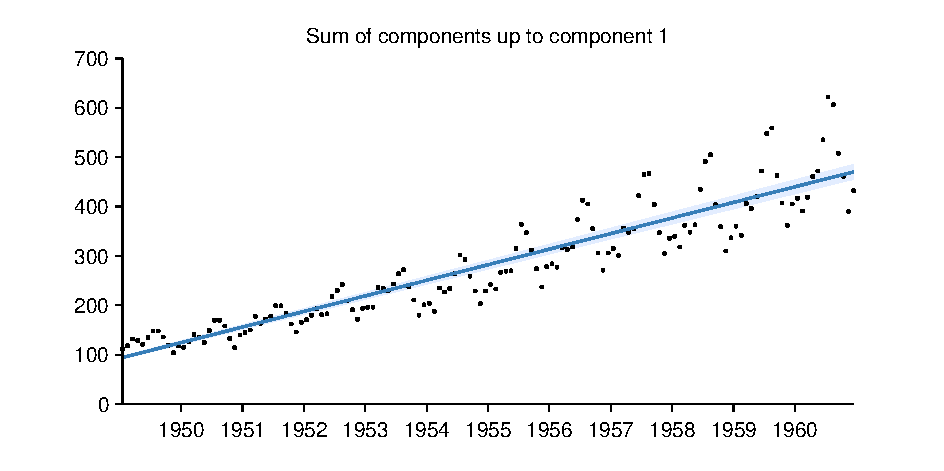
\includegraphics[width=\wmgd,height=\hmgd]{\mdrd/01-airline_1_cum}
\end{tabular}
\end{frame}

\begin{frame}{Example: Airline passenger volume}
\newcommand{\wmgd}{0.5\columnwidth}
\newcommand{\hmgd}{3.0cm}
\newcommand{\mdrd}{figures/01-airline}
\newcommand{\mbm}{\hspace{-0.3cm}}
{\footnotesize
This component is approximately periodic with a period of 1.0 years and varying amplitude.
Across periods the shape of this function varies very smoothly.
The amplitude of the function increases approximately linearly.
The shape of this function within each period has a typical lengthscale of 6.1 weeks.
}

\vspace{\baselineskip}

\begin{tabular}{cc}
\mbm 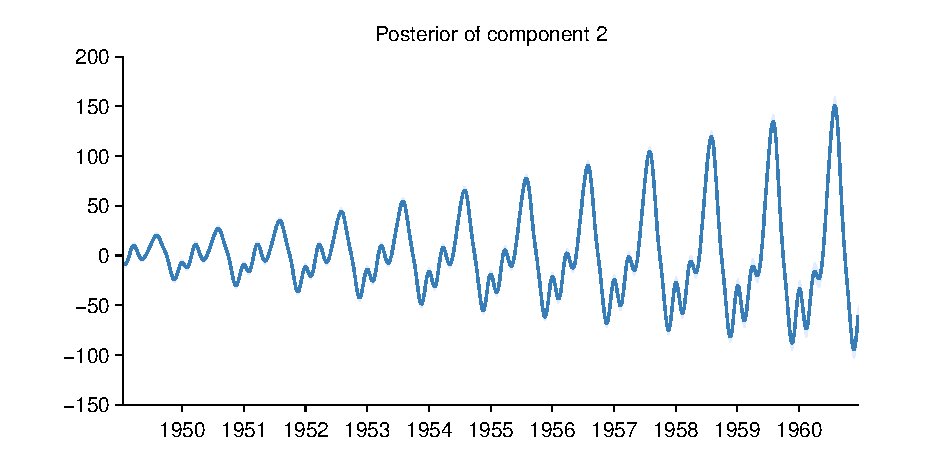
\includegraphics[width=\wmgd,height=\hmgd]{\mdrd/01-airline_2} & 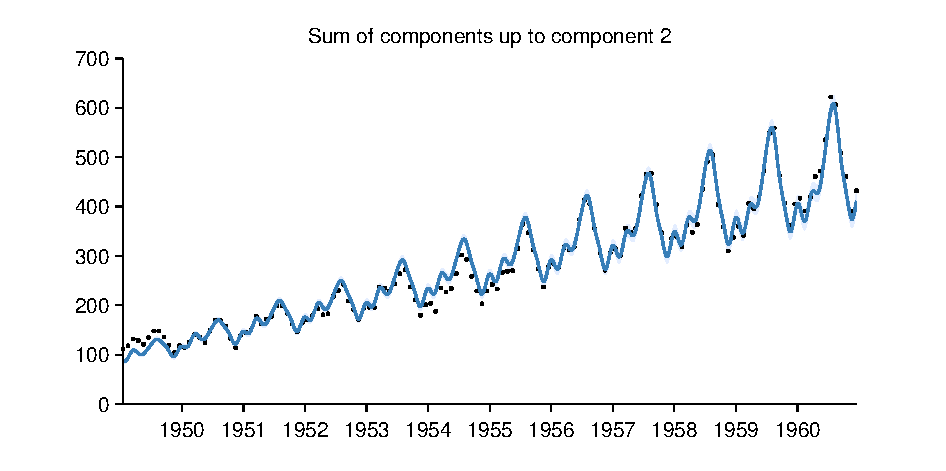
\includegraphics[width=\wmgd,height=\hmgd]{\mdrd/01-airline_2_cum}
\end{tabular}
\end{frame}

\begin{frame}{Example: Airline passenger volume}
\newcommand{\wmgd}{0.5\columnwidth}
\newcommand{\hmgd}{3.0cm}
\newcommand{\mdrd}{figures/01-airline}
\newcommand{\mbm}{\hspace{-0.3cm}}
{\footnotesize
This component is a smooth function with a typical lengthscale of 8.1 months.
}

\vspace{\baselineskip}

\begin{tabular}{cc}
\mbm 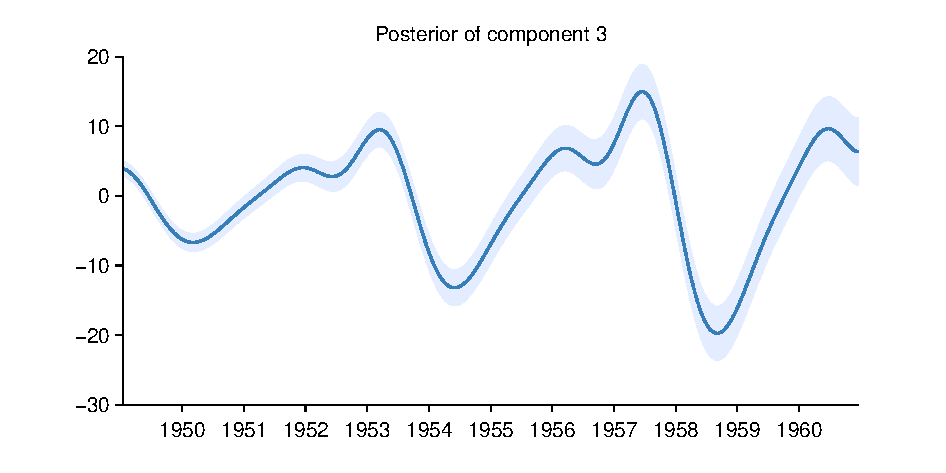
\includegraphics[width=\wmgd,height=\hmgd]{\mdrd/01-airline_3} & 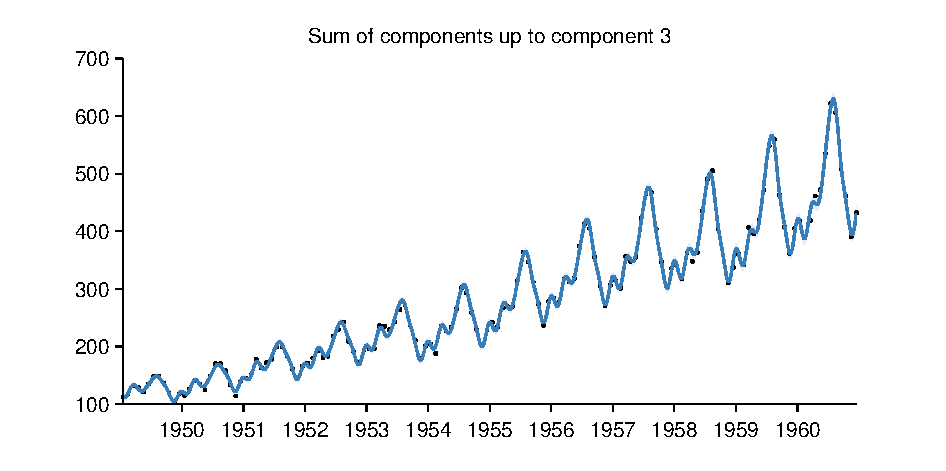
\includegraphics[width=\wmgd,height=\hmgd]{\mdrd/01-airline_3_cum}
\end{tabular}
\end{frame}

\begin{frame}{Example: Airline passenger volume}
\newcommand{\wmgd}{0.5\columnwidth}
\newcommand{\hmgd}{3.0cm}
\newcommand{\mdrd}{figures/01-airline}
\newcommand{\mbm}{\hspace{-0.3cm}}
{\footnotesize
This component models uncorrelated noise.
The standard deviation of the noise increases linearly.
}

\vspace{\baselineskip}

\begin{tabular}{cc}
\mbm 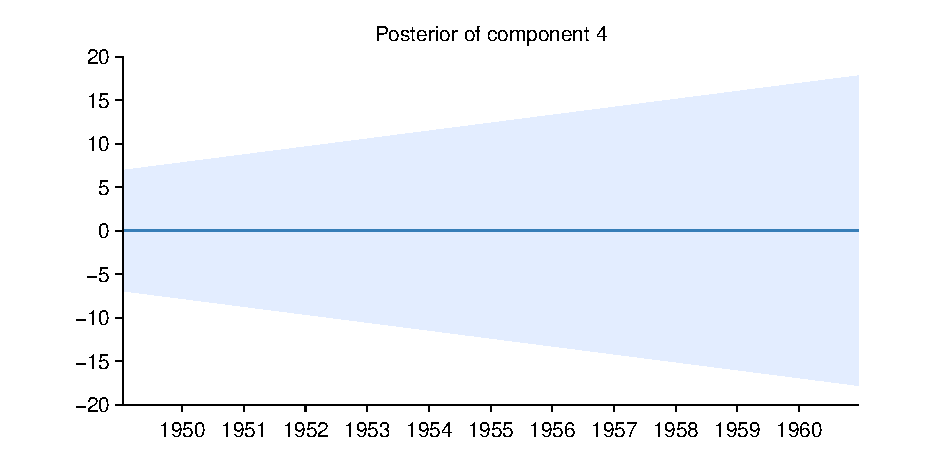
\includegraphics[width=\wmgd,height=\hmgd]{\mdrd/01-airline_4} & 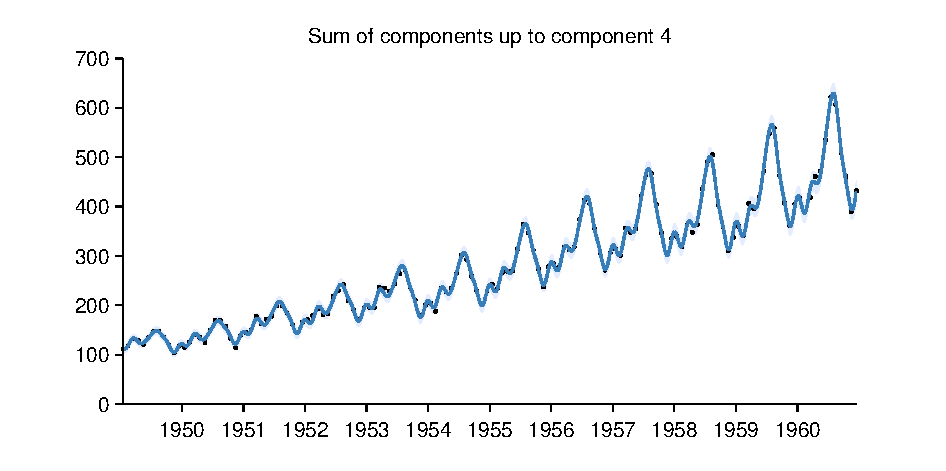
\includegraphics[width=\wmgd,height=\hmgd]{\mdrd/01-airline_4_cum}
\end{tabular}
\end{frame}

\begin{frame}{Example: Solar irradiance}
\newcommand{\wmgd}{0.5\columnwidth}
\newcommand{\hmgd}{3.0cm}
\newcommand{\mdrd}{figures/02-solar}
\newcommand{\mbm}{\hspace{-0.3cm}}
{\footnotesize
This component is constant.
}

\vspace{\baselineskip}

\begin{tabular}{cc}
\mbm \includegraphics[width=\wmgd,height=\hmgd]{\mdrd/02-solar_1} & \includegraphics[width=\wmgd,height=\hmgd]{\mdrd/02-solar_1_cum}
\end{tabular}
\end{frame}

\begin{frame}{Example: Solar irradiance}
\newcommand{\wmgd}{0.5\columnwidth}
\newcommand{\hmgd}{3.0cm}
\newcommand{\mdrd}{figures/02-solar}
\newcommand{\mbm}{\hspace{-0.3cm}}
{\footnotesize
This component is constant.
This component applies from 1644 until 1713.
}

\vspace{\baselineskip}

\begin{tabular}{cc}
\mbm \includegraphics[width=\wmgd,height=\hmgd]{\mdrd/02-solar_2} & \includegraphics[width=\wmgd,height=\hmgd]{\mdrd/02-solar_2_cum}
\end{tabular}
\end{frame}

\begin{frame}{Example: Solar irradiance}
\newcommand{\wmgd}{0.5\columnwidth}
\newcommand{\hmgd}{3.0cm}
\newcommand{\mdrd}{figures/02-solar}
\newcommand{\mbm}{\hspace{-0.3cm}}
{\footnotesize
This component is a smooth function with a typical lengthscale of 23.1 years.
This component applies until 1643 and from 1716 onwards.
}

\vspace{\baselineskip}

\begin{tabular}{cc}
\mbm \includegraphics[width=\wmgd,height=\hmgd]{\mdrd/02-solar_3} & \includegraphics[width=\wmgd,height=\hmgd]{\mdrd/02-solar_3_cum}
\end{tabular}
\end{frame}

\begin{frame}{Example: Solar irradiance}
\newcommand{\wmgd}{0.5\columnwidth}
\newcommand{\hmgd}{3.0cm}
\newcommand{\mdrd}{figures/02-solar}
\newcommand{\mbm}{\hspace{-0.3cm}}
{\footnotesize
This component is approximately periodic with a period of 10.8 years.
Across periods the shape of this function varies smoothly with a typical lengthscale of 36.9 years.
The shape of this function within each period is very smooth and resembles a sinusoid.
This component applies until 1643 and from 1716 onwards.
}

\vspace{\baselineskip}

\begin{tabular}{cc}
\mbm \includegraphics[width=\wmgd,height=\hmgd]{\mdrd/02-solar_4} & \includegraphics[width=\wmgd,height=\hmgd]{\mdrd/02-solar_4_cum}
\end{tabular}
\end{frame}

\begin{frame}{Good predictive performance as well}
  \begin{block}{Standardised RMSE over 13 data sets}
  \includegraphics[width=0.99\textwidth]{figures/box_extrap_wide}\\
  \begin{itemize}
    \item Tweaks can be made to the algorithm to improve accuracy or interpretability of models produced\ldots
    \vspace{\baselineskip}
    \item \ldots but both methods are highly competitive at extrapolation (shown above) and interpolation
  \end{itemize}
  \end{block}
\end{frame}

\begin{frame}{Challenges}
  \begin{itemize}
    \item Interpretability / accuracy
    \vspace{\baselineskip}
    \item Increasing the expressivity of language
    \begin{itemize}
      \item \eg Monotonocity, positive functions, symmetries
    \end{itemize}
    \vspace{\baselineskip}
    \item Computational complexity of searching through a huge space of models
    \vspace{\baselineskip}
    \item Extending the automatic reports to multidimensional datasets
    \begin{itemize}
      \item Search and descriptions naturally extend to multiple dimensions, but automatically generating relevant visual summaries harder 
    \end{itemize}
  \end{itemize}
\end{frame}

\begin{frame}{Current and future directions}
  \begin{itemize}
    \item Automatic statistician for:
    \begin{itemize}
      \item Multivariate nonlinear regression
      \item Classification
      \item Completing and interpreting tables and databases
    \end{itemize}
    \vspace{\baselineskip}
    \item Probabilistic programming
    \begin{itemize}
      \item Probabilistic models are expressed in a general (Turing complete) programming
language (e.g. Church/Venture/Anglican)
      \item A universal inference engine can then be used to infer unobserved variables
given observed data
      \item This can be used to implement seach over the model space in an automated
statistician
    \end{itemize}
  \end{itemize}
\end{frame}

\begin{frame}{Summary}
  \begin{itemize}
    \item We have briefly introduced Bayesian statistics and Gaussian processes
    \vspace{\baselineskip}
    \item Described the beginnings of an automatic statistician for regression
    \begin{itemize}
      \item Defines an open-ended language of models
      \item Searches greedily through this space
      \item Produces detailed reports describing patterns in data
    \end{itemize}
    \vspace{\baselineskip}
    \item We believe this line of research has the potential to make powerful statistical model-building techniques accessible to non-experts
  \end{itemize}
\end{frame}

\begin{frame}{Thanks}
  \begin{center}
  \Huge
  Thanks
  \end{center}
\end{frame}

\begin{frame}{Appendix}
\end{frame}

\begin{frame}{Defining a language of regression models}
  \begin{itemize}
    \item Regression consists of {\bf learning a function} $f: \mathcal{X} \to \mathcal{Y}$ from inputs to outputs from example input / output pairs
    \vspace{\baselineskip}
    \item Language should include {\bf simple parametric forms}\ldots
    \begin{itemize}
       \item \eg Linear functions, Polynomials, Exponential functions
     \end{itemize}
    \vspace{\baselineskip}
    \item \ldots as well as functions specified by {\bf high level properties}
    \begin{itemize}
       \item \eg Smoothness, Periodicity
     \end{itemize}
    \vspace{\baselineskip}
    \item Inference should be {\bf tractable for all models} in language
  \end{itemize}
\end{frame}

\begin{frame}{A language of Gaussian process kernels}
  \begin{itemize}
    \item It is common practice to use a zero mean function since the mean can be marginalised out
  \begin{itemize}
    \item Suppose, ${f(x) \,|\, a \,\sim\, \gp{}(a \times \mu(x), \kernel(x,x'))}$ where $a \,\sim\, \mathcal{N}(0,1)$
    \item Then equivalently, $f(x) \,\sim\, \gp{}(0, \mu(x)\mu(x') + \kernel(x,x'))$
  \end{itemize}
  \vspace{\baselineskip}
  \item We therefore define a language of \gp{} regression models by
specifying a {\bf language of kernels}
  \end{itemize}
\end{frame}

\begin{frame}{Modeling changepoints}
  Assume $\textcolor{red}{f_1(x)} \sim GP(0,k_1)$ and $\textcolor{blue}{f_2(x)} \sim GP(0,k_2)$. Define:
\[
f(x) = (1-\sigma(x)) \textcolor{red}{f_1(x)} + \sigma(x) \textcolor{blue}{f_2(x)}
\]

where $\sigma$ is a sigmoid function between 0 and 1.

\vspace{\baselineskip}

Then $f \sim GP(0,k)$, where
\[
k(x,x') = (1-\sigma(x)) \, \textcolor{red}{k_1(x,x')}  \, (1-\sigma(x')) + \sigma(x) \,
\textcolor{blue}{k_2(x,x')} \, \sigma(x') 
\]

We define the changepoint operator $\kernel = \kCP(\kernel_1, \kernel_2)$.

\vspace{\baselineskip}

  \begin{tabular}{cccc}
    \includegraphics<1>[width=0.2\textwidth]{figures/cp_examples/draw_1} &
    \includegraphics<1>[width=0.2\textwidth]{figures/cp_examples/draw_2} &
    \includegraphics<1>[width=0.2\textwidth]{figures/cp_examples/draw_3} &
    \includegraphics<1>[width=0.2\textwidth]{figures/cp_examples/draw_4}
  \end{tabular}

\end{frame}

\begin{frame}{Model evaluation}
  \begin{itemize}
    \item After proposing a new model its kernel parameters are optimised by conjugate gradients
    \vspace{\baselineskip}
    \item We evaluate each optimised model, $M$, using the \textcolor{red}{marginal likelihood} which can be computed analytically for \gp{}s
    \vspace{\baselineskip}
    \item We \textcolor{blue}{penalise} the marginal likelihood for the \textcolor{blue}{optimised kernel parameters} using the Bayesian Information Criterion (BIC):
\[
-0.5 \times \textrm{BIC}(M) = \textcolor{red}{\log p(D\,|\, M)} - \textcolor{blue}{\frac{p}{2} \log n}
\]
where $p$ is the number of kernel parameters, $D$ represents the data, and $n$ is the number of data points.
  \end{itemize}
\end{frame}

\end{document}

\begin{frame}{Title}
  \begin{itemize}
    \item Content
    \vspace{\baselineskip}
    \item Content
    \vspace{\baselineskip}
    \item Content
    \begin{itemize}
       \item Content
       \item Content
     \end{itemize}
  \end{itemize}
\end{frame}  <onslide
